% Cambridge Battlecode Postmortem
% Formatted with the ACM sigconf (acmart) template with the `nonacm` class option.

\documentclass[10pt,sigconf,nonacm]{acmart}

\makeatletter
\def\@ACM@checkaffil{%
  \if@ACM@instpresent\else
    \ClassWarningNoLine{\@classname}{No institution present for an affiliation}%
  \fi
}
\newcommand{\asseticon}[2]{%
  \begin{minipage}[t]{0.13\textwidth}
    \centering
    \includegraphics[width=0.72\linewidth]{#2}\\[-0.15em]
    {\footnotesize #1}
  \end{minipage}\hfill
}

\let\@vspace\@vspace@orig
\let\@vspacer\@vspacer@orig
\let\@vspace@acm\@vspace@orig
\let\@vspacer@acm\@vspacer@orig
\makeatother

\setcounter{secnumdepth}{0}

\usepackage{float}
\usepackage{xcolor}
\usepackage{listings}
\usepackage{parskip}
\usepackage{enumitem}
\usepackage{subcaption}

\newcommand{\assetbox}[2][0.18\linewidth]{%
  \begin{minipage}[t]{#1}%
    \centering
    \vspace{-0.2em}%
    \includegraphics[width=0.9\linewidth]{#2}%
  \end{minipage}%
}

\newcommand{\assetitem}[3]{%
  \item
  \begin{minipage}[t]{0.74\linewidth}%
    \raggedright
    \textbf{#1:} #2%
  \end{minipage}%
  \hfill
  \assetbox[0.18\linewidth]{#3}%
}

\newcommand{\statefigure}[3]{%
  \begin{figure}[htbp]
    \centering
    \includegraphics[width=0.72\linewidth]{#1}
    \caption{#2}
    \Description{#2}
    \if\relax\detokenize{#3}\relax\else\label{#3}\fi
  \end{figure}
}

\definecolor{kwcol}{RGB}{20,20,150}
\definecolor{cmtcol}{RGB}{95,115,95}
\definecolor{strcol}{RGB}{140,45,45}
\definecolor{bgcol}{RGB}{248,248,248}

\lstdefinestyle{khaos}{
  language=Python,
  basicstyle=\ttfamily\footnotesize,
  keywordstyle=\color{kwcol}\bfseries,
  commentstyle=\color{cmtcol},
  stringstyle=\color{strcol},
  showstringspaces=false,
  breaklines=true,
  breakatwhitespace=true,
  columns=fullflexible,
  keepspaces=true,
  frame=tb,
  framesep=3pt,
  xleftmargin=2pt,
  xrightmargin=2pt,
  backgroundcolor=\color{bgcol},
  numbers=none,
  aboveskip=0.7em,
  belowskip=0.4em,
  literate={->}{{$\rightarrow$}}2 {>=}{{$\geq$}}1 {<=}{{$\leq$}}1
           {!=}{{$\neq$}}1 {&}{{\&}}1
}
\lstset{style=khaos}

\newcommand{\code}[1]{{%
  \def\_{\char`\_\discretionary{}{}{}}%
  \texttt{\small #1}%
}}

\setlength{\emergencystretch}{3em}
\begin{document}

\title[Cambridge Battlecode Postmortem]{Cambridge Battlecode Postmortem}
\subtitle{Team Pantheon}

\author{Derek Wang}
\affiliation{%
  \vspace{-0.4em}%
  \institution{University of Oxford}%
}
\author{Yufan Wang}
\affiliation{%
  \vspace{-0.4em}%
  \institution{Georgia Institute of Technology}%
}
\author{Alex Thummalapalli}
\affiliation{%
  \vspace{-0.4em}%
  \institution{Georgia Institute of Technology}%
  \vspace{1.5em}%
}
\author{Ioannis Pantidis}
\affiliation{%
  \vspace{-0.4em}%
  \institution{Delft University of Technology}%
  \vspace{1.5em}%
}

\renewcommand{\shortauthors}{Wang et al.}

\maketitle


\section{Overview}

We competed in the inaugural Cambridge Battlecode as Team
Pantheon, consisting of Derek Wang, Yufan Wang, Alex
Thummalapalli, and Ioannis Pantidis.

We entered the competition with mixed levels of experience. For three
of us, this was our first year doing Battlecode.
Ultimately, we placed first in the Grand Finals with our
bot, Khaos. The final bot, along with our tooling, can be found in
our \href{https://github.com/HerbertTheBird/Cambridge-Battlecode}{GitHub repository}.

\begin{figure}[htbp]
  \centering
  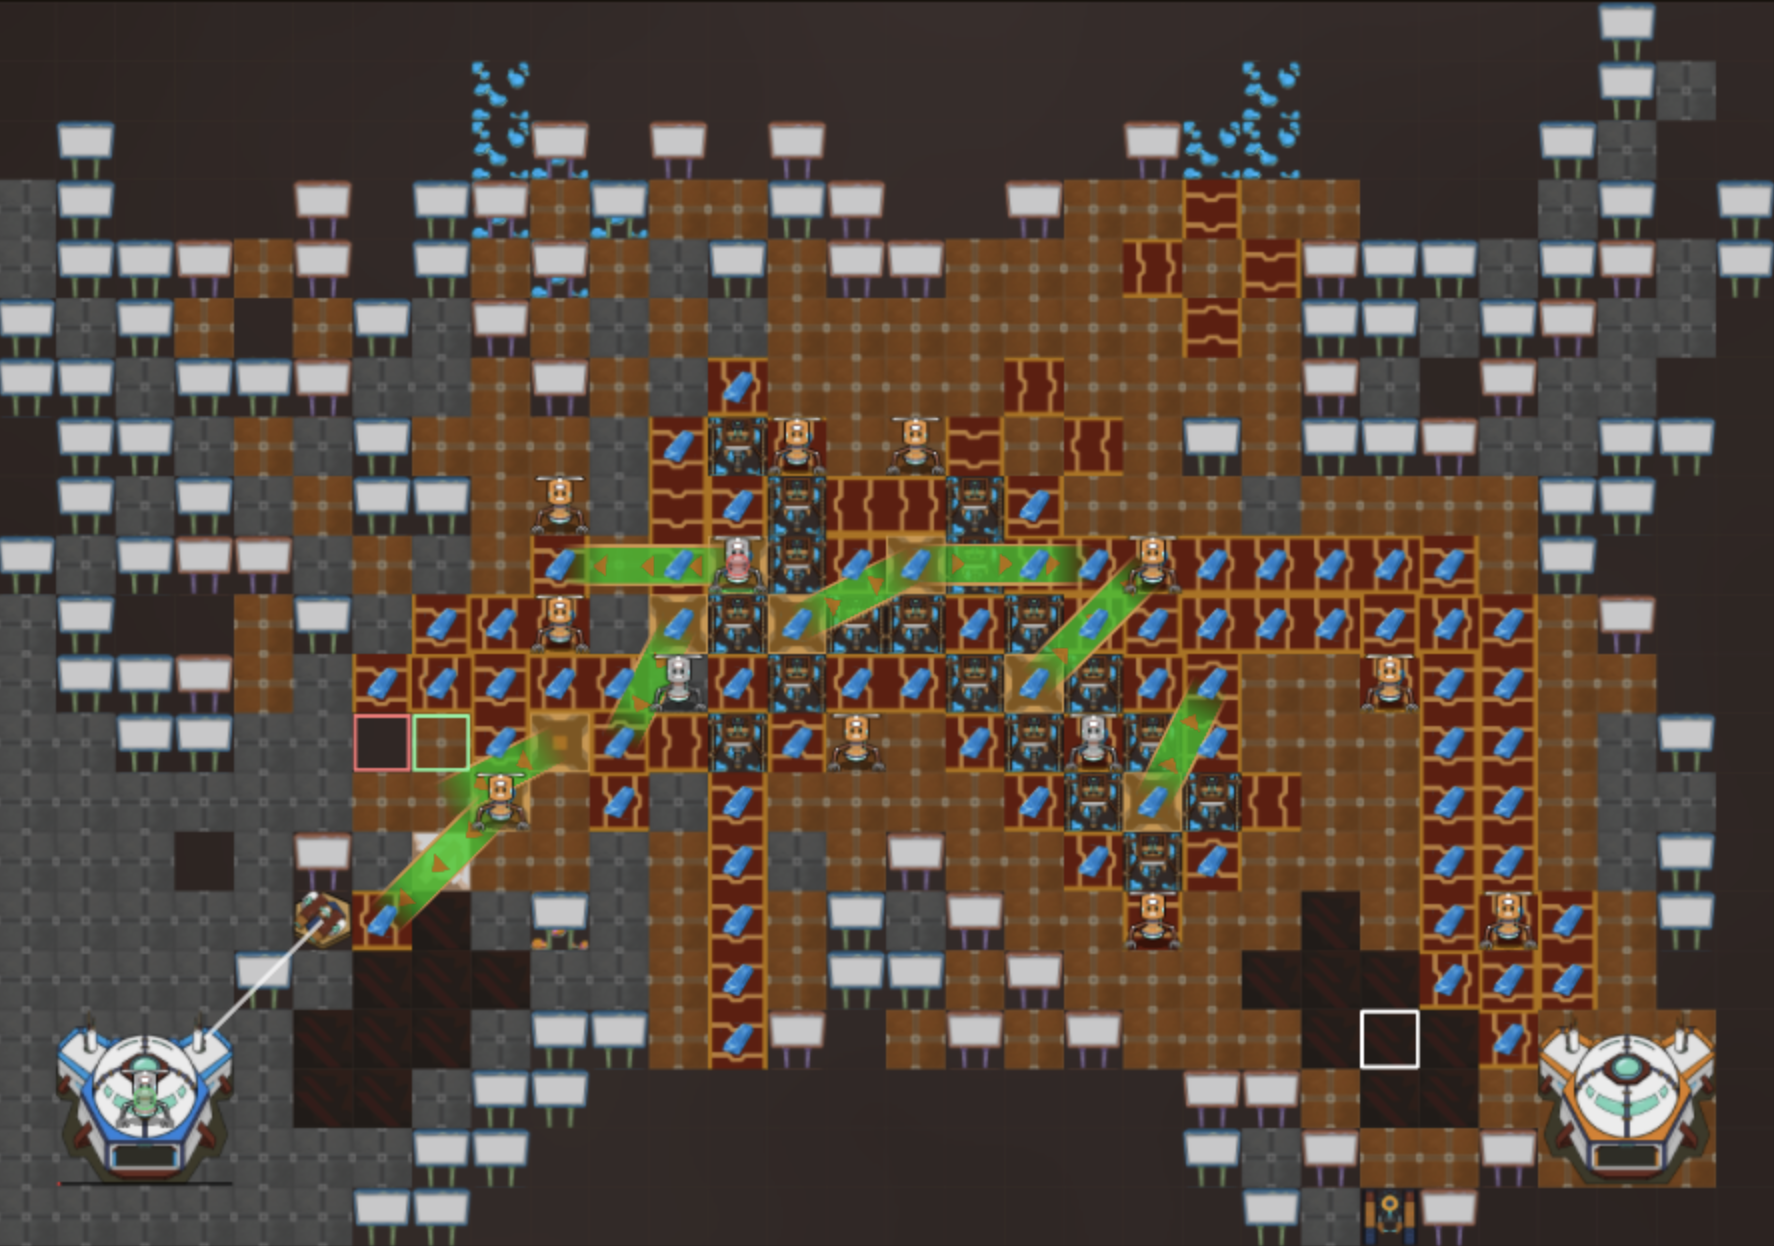
\includegraphics[width=\linewidth]{images/cambridge_battlecode.png}
  \caption{A Grand Finals match between Pantheon (gold) and something else (silver).}
  \Description{Screenshot of a Cambridge Battlecode match showing Pantheon's gold-colored bots and infrastructure facing an opposing silver team on the game map.}
\end{figure}


\section{Game Overview}

Cambridge Battlecode is a six-week competition in which teams design
and develop algorithms to autonomously play a turn-based strategy
game. This year's game involved balancing resource management, map
control, and combat by dynamically routing conveyor lines across a 2D
map.

Though it was inspired by MIT Battlecode, this competition featured some key differences; notably, a switch from Java to Python, new time limit constraints in place of bytecode counting, and a large jump in complexity.

Each match is played on a rectangular map, ranging in size from $20 \times 20$ to $50 \times 50$ and guaranteed to be horizontally, vertically, or rotationally symmetric. Each team starts with a single core unit that can spawn builder bots, each running an independent copy of the same program.

Though the map is initially composed of four basic tile types (empty, titanium ore, axionite ore, walls), builder bots can construct new infrastructure throughout the game such as conveyors, turrets, and roads.


\begin{figure}[htbp]
  \centering
  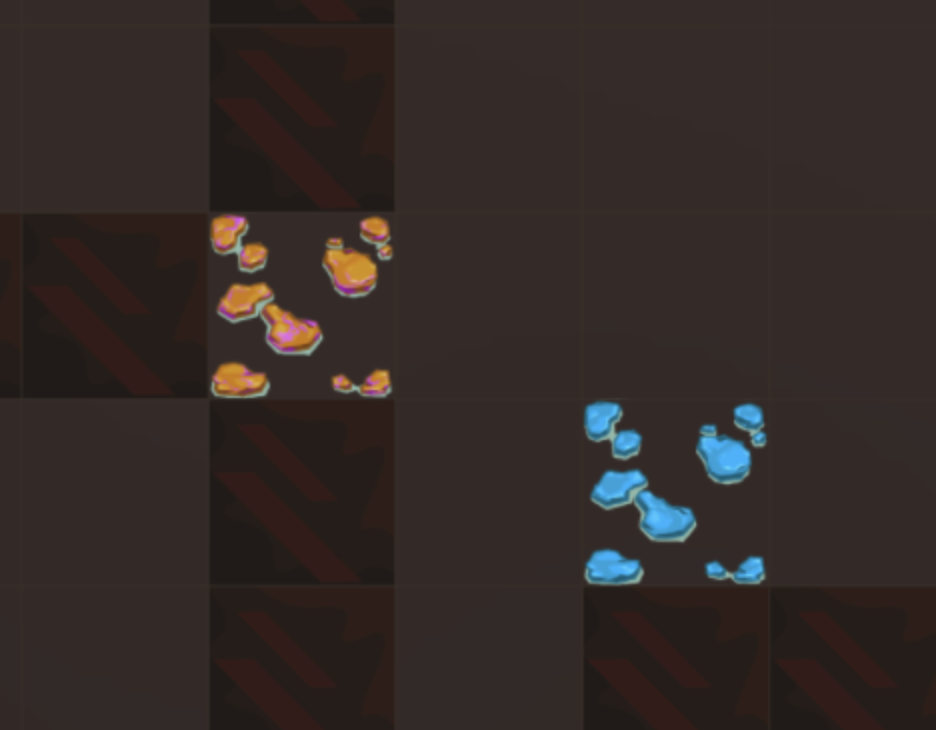
\includegraphics[width=0.8\linewidth]{images/map_features.png}
  \caption{Map features: titanium ore in blue, axionite ore in
    orange, and walls in black.}
  \Description{A Battlecode map illustrating the four basic tile types: empty tiles, titanium ore shown in blue, axionite ore shown in orange, and walls shown in black.}
\end{figure}

\subsection{Resources}
Titanium is the primary resource and is used to build buildings, heal, and
as ammunition for most turrets. Raw axionite is what is mined from axionite ore. Raw axionite and titanium can be combined to create refined axionite (typically referred to as simply ``axionite''), which is a premium resource with more limited uses,
although it can be converted back into titanium or used for tiebreaks.
\vfill\null




\begin{figure*}[t]
  \centering

  \asseticon{Core}{images/core.png}
  \asseticon{Builder Bot}{images/builder-bot.png}
  \asseticon{Conveyor}{images/conveyor.png}
  \asseticon{Armoured Conveyor}{images/armoured-conveyor.png}
  \asseticon{Bridge}{images/bridge.png}
  \asseticon{Splitter}{images/splitter.png}
  \asseticon{Harvester}{images/harvester.png}

  \vspace{0.8em}

  \asseticon{Foundry}{images/foundry.png}
  \asseticon{Gunner}{images/gunner.png}
  \asseticon{Sentinel}{images/sentinel.png}
  \asseticon{Breach}{images/breach.png}
  \asseticon{Launcher}{images/launcher.png}
  \asseticon{Road}{images/road.png}
  \asseticon{Barrier}{images/barrier.png}

  \caption{Game entities and buildings.}
  \Description{In-game screenshots of the various buildings and units.}
\end{figure*}

\subsection{Core}

Each team starts with a core, placed symmetrically on opposite sides of the map.
The core is an immobile $3 \times 3$ building.

It can spawn builder bot units on one of its tiles once per turn, and it is walkable only by
allied builder bots.

Resources must be delivered to the core before they become globally accessible to all units.
The core also has the ability to convert axionite to titanium in a 1:4 ratio.

\subsection{Builder Bots}

The primary unit in the game is the builder bot. It is the only unit that can move or construct buildings.

Builder bots can move once per turn to an adjacent tile with a walkable building on it.
They can also perform an action once per turn to heal an adjacent entity, construct a building on an adjacent tile, or attack a building on the tile they occupy.
Builder bots can also freely destroy adjacent ally buildings without using up their action.

Builder bot vision extends to squared Euclidean distance $20$.

\subsection{Conveyors}

\begin{itemize}[leftmargin=*]
  \item \textbf{Conveyors} send resources to the tile in front of them. They accept resources from the three cardinal non-facing sides.

  \item \textbf{Armoured conveyors} act like regular conveyors but have more health and cannot be damaged by builder bots. They cost both titanium and axionite to build.

  \item \textbf{Bridges} are more expensive than conveyors but have more output options: any tile within squared distance $\leq 9$. They accept resources from any side.

  \item \textbf{Splitters} only accept resources from behind, but they send outputs equally to the three remaining cardinal sides.
\end{itemize}

\subsection{Economic Buildings}

\begin{itemize}[leftmargin=*]
  \item \textbf{Harvesters} can be built on titanium or axionite ore to harvest resources. They output resources every four turns to a cardinally adjacent building, like a conveyor or turret.

  \item \textbf{Foundries} convert titanium and raw axionite into refined axionite. They accept input from any side and will output refined axionite after consuming both types of input resources.
\end{itemize}

\subsection{Turrets}

Turrets are the primary way of attacking. All turret types except launchers require ammo to fire, meaning resources must be fed into them from a non-facing side. There are four types of turrets:

\begin{itemize}[leftmargin=*]
  \item \textbf{Gunners} are high-DPS, low-range turrets that can only shoot the first target in range. They can turn by spending titanium.

  \item \textbf{Sentinels} are lower-DPS turrets with a long and wide range. Unlike gunners, they can shoot any tile within their range.

  \item \textbf{Breaches} are very high-DPS turrets that deal splash damage. However, they can only use refined axionite as ammo, so they are seldom used.

  \item \textbf{Launchers} are utility turrets that can pick up and launch adjacent builder bots on either team to any walkable tile in their vision.
\end{itemize}

\subsection{Miscellaneous Buildings}

\begin{itemize}[leftmargin=*]
  \item \textbf{Roads} are cheap, walkable buildings. Since builder bots cannot walk on empty tiles, a road must be placed before that tile is passable.

  \item \textbf{Barriers} are cheap, high-health buildings that block builder movement.
\end{itemize}
\subsection{Winning the Game}

There are two win conditions: either destroying the enemy core or winning by tiebreak after 2000 rounds have passed. Tiebreakers are determined in order:

\begin{itemize}[leftmargin=*]
  \item Axionite collected
  \item Titanium collected
  \item Harvesters alive
  \item Axionite stored
  \item Titanium stored
\end{itemize}

\section{Bot Summary}

We went through several substantial iterations and even entire rewrites over the course of the competition.

\subsection{Starter}
\statefigure{images/starter.png}{Starter (Gold) vs Starter (Silver)}{fig:starter}
We started with a basic economy bot with A* pathfinding, conveyor routing, and minimal attacking.
\subsection{Artemis}
\statefigure{images/artemis.png}{Artemis (Gold) vs Starter (Silver)}{fig:artemis}
Our initial baseline evolved into a launcher-centric bot named Artemis.

A dedicated builder bot would rush the enemy core using launchers to launch itself forward in hopes of disrupting their early economy very quickly. Then it would find a conveyor to attempt to attack
and replace with a turret to destroy the enemy core. It would place additional launchers to fling away any enemy
builder bot attempting to heal the tile the rusher was attacking.

Artemis also used a defensive launcher network both to protect our conveyors and harvesters and to help
ally bots quickly move across the map.



\subsection{Demeter}
\statefigure{images/demeter.png}{Demeter (Gold) vs Artemis (Silver)}{fig:demeter}
After merging with Team Food, we bug-fixed Alex's bot and ported over our map info, pathfinding, and gunner logic from Artemis.
This defensive bot solely focused on developing infrastructure, but also had dynamic
turret placement logic that would repurpose our own conveyor lines if they
were needed more for defense. However, we soon hit a plateau due to overcomplicated code and strategies
and had to begin a rewrite.


\subsection{Lethe}
\statefigure{images/lethe.png}{Lethe (Gold) vs Demeter (Silver)}{fig:lethe}
Keeping only our map info and pathfinding modules, we fully rewrote our bot with a memoryless
architecture. The idea behind the memoryless system was to have our bot recompute information
every turn based on global map knowledge, rather than retaining stale strategies or states.
This allowed our bot to be highly dynamic and make much more optimal decisions each turn, and
we finally started winning games against top teams like Blue Dragon.

\subsection{Hades}
\statefigure{images/hades.png}{Hades (Gold) vs Lethe (Silver)}{fig:hades}

After the US Qualifiers, we added many small improvements and partial rewrites to Lethe. We also
revamped our coordination system, which previously used markers for bot coordination, since it was being
disrupted by other teams placing roads everywhere and blocking marker placement spots. The new system
used factors like closest builder to a target tile to decide whether to pursue a task.


\subsection{Khaos}
\statefigure{images/khaos.png}{Khaos (Gold) vs Hades (Silver)}{fig:khaos}

A day before the final submission deadline, we merged in a brand new chokepoint detection system
and attack route strategy that greatly improved our win rate. We named this bot Khaos due to its
unpredictable and dynamic nature, which made it difficult for opponents to counter.

\section{Strategic Overview}

The rest of this postmortem documents how Khaos works. We'll start with general strategies, then
cover technical implementation from the map info layer through pathfinding, states, turret logic, and runtime optimization.

\subsection{Memoryless Architecture}

Our bitmasked map info layer is fast enough for us to recompute key decision-making and planning logic from scratch each turn. Rather than defining state transitions based on previous states, we score seven candidate states each turn based on current map knowledge and execute the highest scoring state.

The intent is for long-term behavior to emerge from every builder acting optimally on its current local knowledge. This makes each bot's actions much more dynamic, since they don't persist stale goals and can easily adapt to the actions of other bots, newly discovered information, etc.

\subsection{Adversarial Strategies}

Although these territorial strategies are not hard-coded, they emerge
from our state management and scoring system and are worth highlighting.

\textbf{Ore hopping} is our strategy of using ally-controlled harvesters as staging points
for attack turrets. By placing turrets along the frontier of our controlled territory, we
can shoot the defenses around nearby opponent harvesters. Our builder bots can then take over
the enemy harvester by building more turrets around it.

Ore hopping is a consistent way of pushing our front line forward,
since slowly taking over enemy harvesters bolsters our economy and increases map control. This often will create turret combat along the frontier.

The only downside of ore hopping is that it is highly dependent on ore spread across the map. If ore clumps aren't spread
out enough, a turret placed at an ally ore cannot reach an enemy ore, and it is harder to hop and meaningfully expand our territory.

\begin{figure}[htbp]
  \centering
  \begin{minipage}{0.46\linewidth}
    \centering
    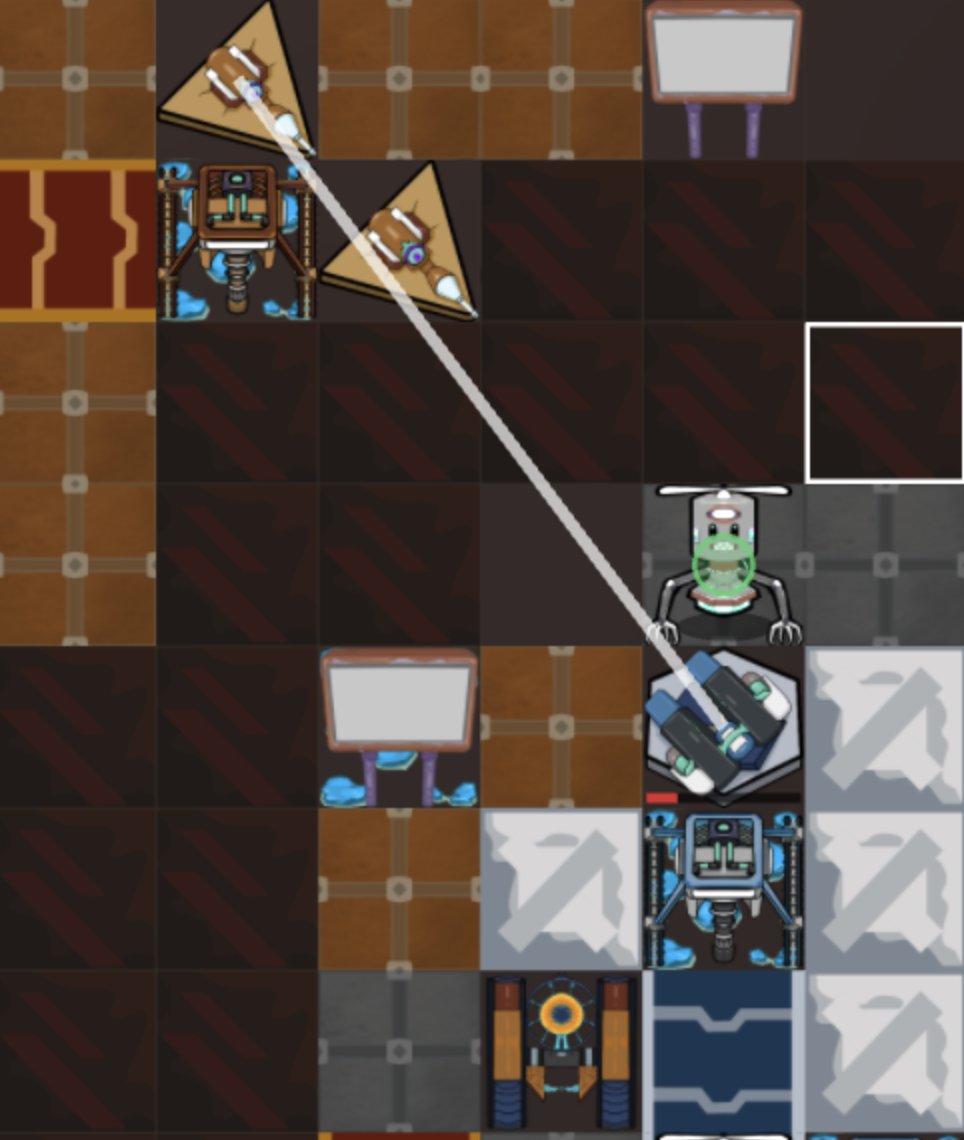
\includegraphics[width=\linewidth]{images/ore_hop_before.png}\\
    {\small Before}
  \end{minipage}
  \hfill
  \begin{minipage}{0.46\linewidth}
    \centering
    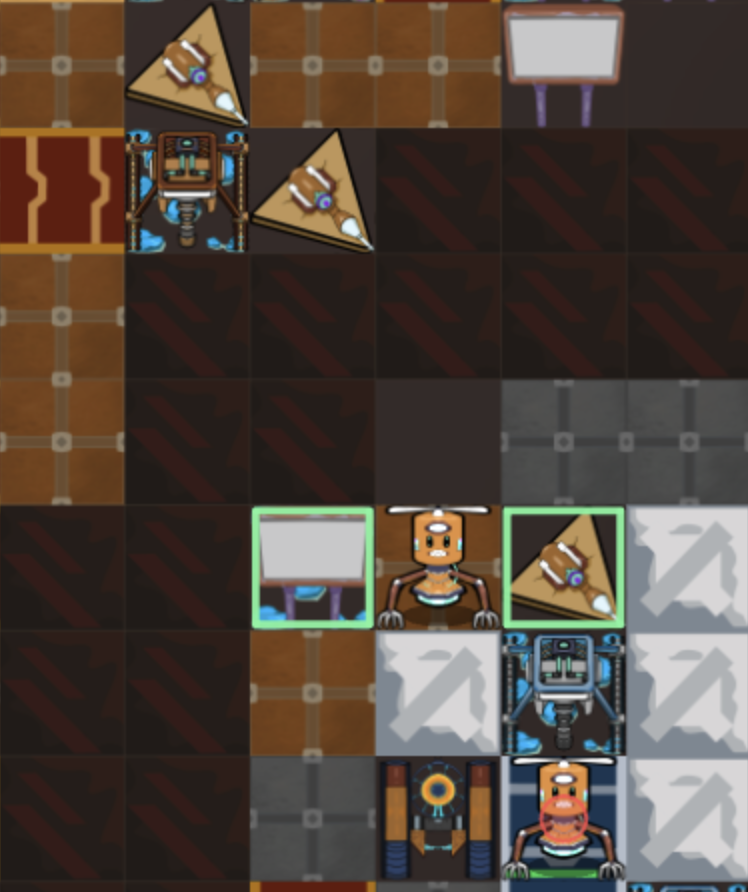
\includegraphics[width=\linewidth]{images/ore_hop_after.png}\\
    {\small After}
  \end{minipage}
  \caption{Ore hopping.}
  \Description{Two side-by-side game screenshots showing the ore-hopping strategy: in the ``before'' image, friendly turrets sit along the frontier of our territory; in the ``after'' image, those turrets have eliminated an enemy gunner adjacent to a nearby enemy harvester, allowing us to take it over.}
\end{figure}


\textbf{Seeding} is a more aggressive way of gaining territory. This involves
builder bots intercepting an enemy conveyor line by attacking it until an allied ``seed'' turret can be placed in the gap. The analogy is that much like seeding a plant, our infrastructure can grow from a single turret investment as it destroys enemy targets around it and frees up space for more of our turrets and conveyors to be placed.

Seeding is easily countered by enemy builder bots simply out-healing the attack if nearby, though there are special cases described later where this can be prevented.

\begin{figure}[htbp]
  \centering
  \begin{minipage}{0.46\linewidth}
    \centering
    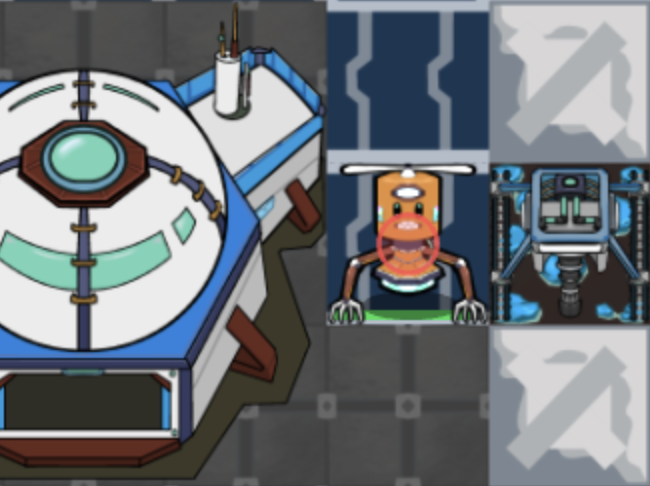
\includegraphics[width=\linewidth]{images/seeding_before.png}\\
    {\small Before}
  \end{minipage}
  \hfill
  \begin{minipage}{0.46\linewidth}
    \centering
    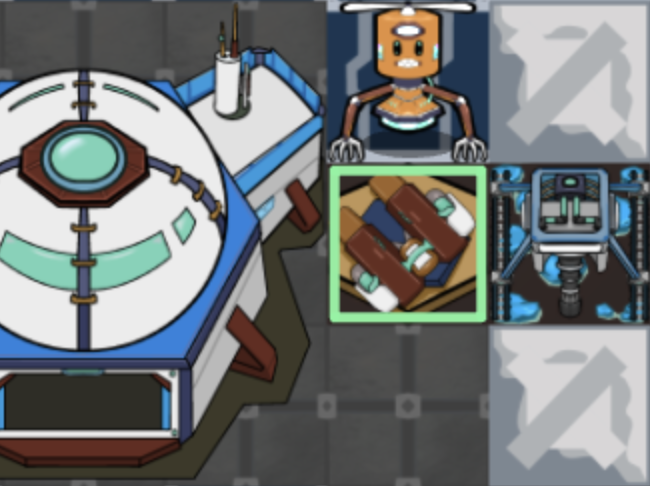
\includegraphics[width=\linewidth]{images/seeding_after.png}\\
    {\small After}
  \end{minipage}
  \caption{Seeding.}
  \Description{Two side-by-side game screenshots showing the seeding strategy: in the ``before'' image, a builder bot attacks an enemy conveyor line to create a gap; in the ``after'' image, an allied ``seed'' turret has been placed in that gap.}
\end{figure}

\section{Map Info}

The map is at most $W\!\times\!H \le 50\!\times\!50$ tiles, so we can fit binary information
about tiles within a Python big integer of at most $2500$ bits. We encode information
about tile $(x,y)$ in bit $n = x + yW$. By using big integers for various properties
(whether a tile is a wall, if we've visited a tile, etc.), we can quickly query and compose spatial information
about the map with C-level bitwise operations.

We frequently use geometric translations of a set of tiles
by using the integer shifts $\ll\!1$, $\gg\!1$, $\ll\!W$, $\gg\!W$ to shift a tile set east, west, south, north respectively.
These geometric translations are useful for shifting bitmasked frontiers, computing neighborhoods/zones, etc.

Overall, \code{map\_info} maintains around thirty derived masks to store information about:

\begin{itemize}
  \item Environment/Entity type
  \item Facing direction
  \item Current/previous visibility
  \item Resource flow
  \item Danger zones
  \item Placement legality
\end{itemize}

We can combine these masks to query various relevant subsets of the board. For example, an avoid mask can be quickly computed by ORing walls, enemy turret threat masks, and some buildings.

Values that cannot be a single bit are stored in Python lists indexed by $n$: building id, entity type, hit
points, facing, conveyor output tile, and a reverse-adjacency bitmask of
every conveyor-type building that outputs onto $n$. That reverse
adjacency of the conveyor graph allows for very fast conveyor flow related calculations.

\subsection{Updating Vision}

\code{update\_at(pos)} calls the cambc controller to update our knowledge of a specific tile.
It is called for every tile in our vision. We also call it on relevant tiles after we build something or when new tiles enter our vision after moving.

Since this method is called so frequently, we only update relevant info to avoid wasting runtime on unneeded controller calls:

\begin{enumerate}
  \item Core-area tiles are handled by separate core logic; only core health is refreshed each turn and the function returns early.
  \item Symmetry tracking runs once per newly-seen tile.
        Observing a tile that contradicts a symmetrical counterpart clears
        that symmetry flag.
  \item Walls can never hold a building and never change, so if the observed tile is a wall, the function returns before the building lookup.
  \item Otherwise, we check the building id. If it is unchanged from last turn, we only refresh health and stored resources, as well as facing direction for gunners (the one unit that turns).
  \item If the building id changed or was cleared, we update all of our bitmasks with the new entity info and bump the structural version counter so any cached calculations that rely on map info are marked stale. For markers, we add their decoded message into the message queue.
\end{enumerate}

\subsection{Predicting Symmetry}

Since maps are guaranteed to be either horizontally, vertically, or rotationally symmetric, we look for tiles that contradict each possible symmetry until there is only one remaining candidate. We then use the determined symmetry to set the enemy core location and update our knowledge about unseen tiles:

\begin{lstlisting}
if (hor + ver + rot) == 1 and not solved_sym:
    solved_sym = True
    # update enemy core location
    their_core = flip(my_core)
    # mirror seen tile envs to unseen half
    for n in seen_tiles:
        f = flipped_index(n)
        if not (seen & bit(f)):
            copy_env(n -> f); seen |= bit(f)
    struct_version += 1
\end{lstlisting}

If there are two or more possible symmetries, we still commit to a prediction on where the enemy core is. We default to assuming rotational symmetry unless it's already been eliminated, in which case we predict the closer of the horizontally or vertically symmetrical core locations, with the tiebreak remembered so the prediction doesn't oscillate between turns. This predicted location is used to predict ally vs enemy territory and for attack routing.

\subsection{Memoization}

We memoize complex bitmasks based on a struct version counter that is incremented on structural changes to the known map (wall discovered or building discovered / placed / destroyed).

For some masks, we also add our observed resource bitmasks to the cache key so that the masks are recomputed as resources flow:

\begin{lstlisting}
cache_key = (_struct_version, 
             _bm_conv_ti, 
             _bm_conv_raw_ax, 
             _bm_conv_refined)
\end{lstlisting}

\subsection{Derived Masks}

We use our basic map info masks to derive more complex masks for decision making.


\textbf{Enemy turret threat:} We compute both a soft mask (enemy sentinel attack tiles) and a hard mask (enemy gunner / breach attack tiles) to guide builder decisions.

We purposely never step within hard mask tiles due to the higher DPS of gunners and breaches. We allow stepping into soft mask tiles in our pathfinding, just at a higher cost.

To construct these masks, we precompute the attack patterns of sentinels and breaches for each facing direction, then apply these patterns for turrets facing each direction:

\begin{lstlisting}
for d in 8 directions:
    turrets_d = enemy_turrets & dir_mask[d]
    for (dx,dy) in OFFSETS[turret_type][d]:
        acc |= shift(turrets_d & col_mask, dx + dy*W)
\end{lstlisting}

Since gunners can only shoot the first tile in front of them, we check their facing direction one step at a time, ignoring any tiles past a blocking wall.

The hard and soft masks are memoized on \code{\_struct\_version} to minimize recomputation.

\textbf{Turret feed propagation:} We construct a bitmask to mark which tiles are properly fed. We propagate whether a tile is fed from harvesters, foundries, and conveyors with visible resources on them up to 4 steps downstream (based on output tiles). This bitmask is used for turret placement logic to only consider tiles with a source of titanium or refined axionite feeding them.


\textbf{Route targets and dead ends:} One pass walks the conveyor graph backward from the core area via
the reverse adjacency, in layers, recording both the reached set and a
topological-ish visit order. A second pass then overlays loaded and
visible state:
\vfill\null

\begin{lstlisting}
reaches_core, order = route_reaches_core()
# walk in core-ward order
for n in order:
    rl = (run_len[target(n)] + 1
          if loaded(n) else 0)
    run_len[n] = rl
    if rl == 4:  # 4 in a row: line jammed
        mark 4 tiles from n unroutable
# a *visible* 4-run jams the whole chain:
# flood both up- and downstream through
# my conveyors
route_targets = core_area | (reaches_core
                 & ~unroutable
                 & ~guard_conveyor)
\end{lstlisting}

If we observe 4 loaded conveyors in a row, we consider that conveyor line
unroutable, and ignore it in our Dijkstra's for conveyor route planning.
This approximates max flow since we don't want to connect more harvesters to a route
that is already full.

As a side effect, the same pass sets a dead-end mask (targets
of loaded conveyors whose output is not an accepting building, plus
conveyors pointing into enemy hard buildings) and a feeding-enemy mask
(loaded conveyors whose target is an enemy
turret). The route state attempts to route dead-ends and feeding-enemy conveyors to routable targets.

We also have a visible-graph check for whether a turret could possibly
still be fed. This check is used by turrets to decide
self-destruction validity: any unseen adjacent tile or off-screen upstream feeder
keeps the answer \code{True}, so a turret is only allowed to self-destruct when the visible
local structure \emph{proves} it is not currently supplied.

\textbf{Carrying resources:} We also maintain a bitmask that expands three steps up and downstream from a resource-carrying conveyor. We maintain separate bitmasks for each resource type so we can check if a tile could carry a particular resource.

\textbf{Avoid pathing:} We also maintain a mask of tiles we should avoid when pathfinding. Our universal avoid mask includes walls, non-walkable buildings, tiles around enemy launchers, and tiles covered by enemy turrets. We can also compute avoid masks that include ally conveyors (so we don't change existing infrastructure when planning a new conveyor route), enemy roads adjacent to enemy bots (since they are easily healable), chokepoint barriers, and non-landlocked ore in the harvest zone.

We also have an enemy POV mode to calculate avoid masks with inverted perspective (shows how the enemy
would perceive tiles to avoid).

\section{Communication}

Since robots are sandboxed, all communication must be relayed via markers.
A unit may place at most one marker per turn carrying a \code{u32} value.

\subsection{Payload Format}

Earlier iterations also used markers to communicate task claims between
builders and to use launchers to speed up builder bot movement, but those were retired in Hades.
The symmetry-broadcast payload repurposed the lower bits as a
$7$-bit \emph{corresponding-position} code, a $21$-bit environment sample,
and $3$ symmetry bits.

All field widths and shifts are module constants and the
encode/decode pair is a straight bit-pack:

\begin{lstlisting}
def encode(target, type, sym, sender):
    return ((target & POS_MASK)
            | (sym    << SYM_SHIFT)
            | (sender << SENDER_SHIFT)
            | (type   << TYPE_SHIFT)) ^ key
\end{lstlisting}

The final XOR with \code{key} encrypts our markers. We initially added this as a joke. However, we kept it in to make it harder for teams to decode markers in replays to figure out how our comms system works.

\subsection{Symmetry Broadcasts}

Although the primary purpose of this marker type is to share map symmetry,
we also use it to share map knowledge about distant parts of the map.

We first bucket the map into
$5\times5$ cells. Since map dimensions are at most $50\times50$, there are up to $100$ buckets, and so we can
communicate which bucket we are sharing info about with $7$ bits. We then use $21$ bits to communicate binary information
about $21$ tiles within the bucket (all tiles within squared radius $\le 5$ from the center of the bucket). If the marker is placed on an even $x$ coordinate, we communicate whether or not the tile environment is a wall. Otherwise, we communicate whether or not it is a titanium ore. This results in each type being communicated by roughly half of our markers.

Any ally bot that reads the marker then uses the learned info to update the corresponding \code{\_bm\_env} entry
and \code{\_bm\_seen}:

\begin{lstlisting}
def apply_symmetry_broadcast_map(marker_pos, bucket, bits):
    env = ORE_TI if marker_pos.x & 1 else WALL
    for i in set_bits(bits):
        dx,dy = LEARN_MAP_OFFSETS[i]
        note_env(bucket.x+dx, bucket.y+dy, env)
\end{lstlisting}

Walls are the more valuable of the two payload types, since knowledge of
impassable tiles helps our pathfinding and chokepoint detection logic. Titanium ore
observations don't affect these since ore is passable, but it does help for more efficient
harvesting since we know where harvesters should be placed before exploring the map.

Overall, our communication system is supplementary only. Bots don't depend on communicated info,
but they can benefit from using markers to learn more of the map.


\section{Pathfinding}

We run a bitmasked version of Dial's algorithm to find the optimal path to a given target. By changing the allowed steps and cost, we can use this both for builder bot movement and conveyor route planning.

The search is run in reverse, from target tiles to start, so that path reconstruction is not necessary, as it can simply find the lowest distance-to-target tile it can move onto.

\subsection{Dijkstra's for Movement}

For movement, we define four different edge types: a normal step (cost 1), a step destroying an ally barrier (cost 15), a step into a soft threat (cost 20), and both (cost 35).

We consider any walls or non-walkable buildings to be impassable. We do not mark builder bots as impassable to prevent oscillations in our route path as bots move around. Instead, we only check occupancy at the end of our Dijkstra's, when considering the move we would make this turn.

We then use a circular array of frontier bitmasks as a bucket queue, starting from a mask of our target tiles and iterating until we reach a tile we could move onto this turn:
\begin{figure}[H]
  \centering

  \begin{subfigure}{0.31\linewidth}
    \centering
    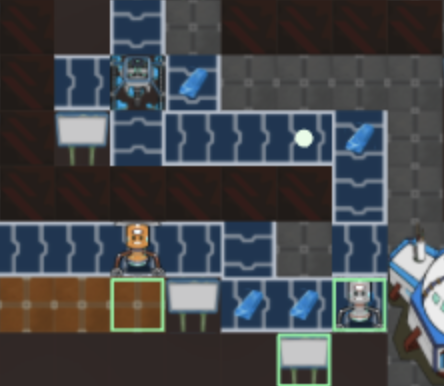
\includegraphics[width=\linewidth]{images/bfs_1.png}
  \end{subfigure}
  \hfill
  \begin{subfigure}{0.31\linewidth}
    \centering
    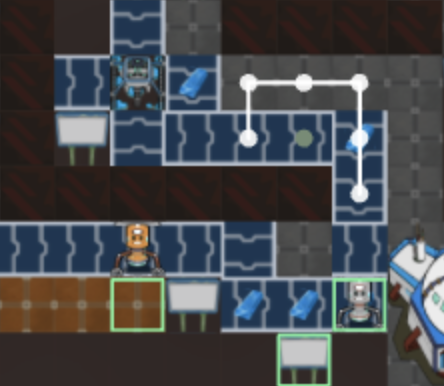
\includegraphics[width=\linewidth]{images/bfs_2.png}
  \end{subfigure}
  \hfill
  \begin{subfigure}{0.31\linewidth}
    \centering
    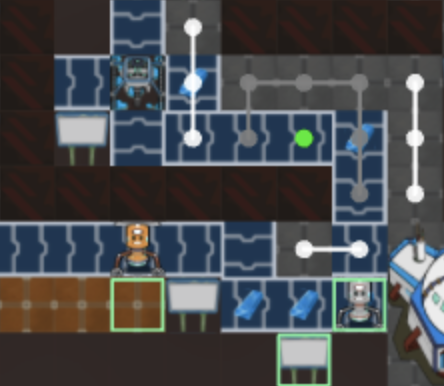
\includegraphics[width=\linewidth]{images/bfs_3.png}
  \end{subfigure}

  \vspace{0.5em}

  \begin{subfigure}{0.31\linewidth}
    \centering
    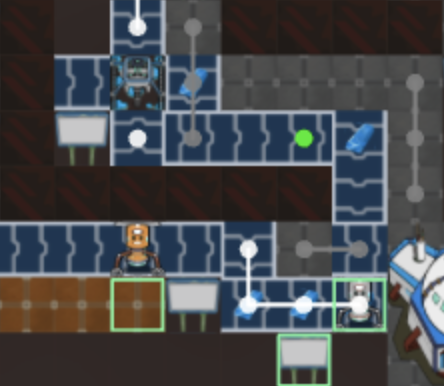
\includegraphics[width=\linewidth]{images/bfs_4.png}
  \end{subfigure}
  \hfill
  \begin{subfigure}{0.31\linewidth}
    \centering
    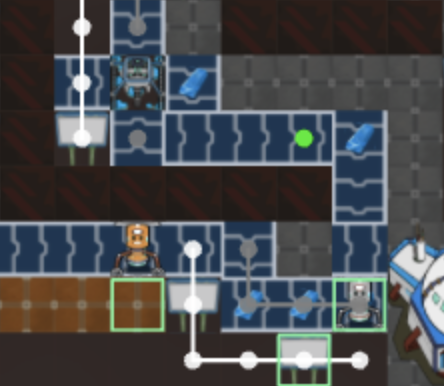
\includegraphics[width=\linewidth]{images/bfs_5.png}
  \end{subfigure}
  \hfill
  \begin{subfigure}{0.31\linewidth}
    \centering
    \phantom{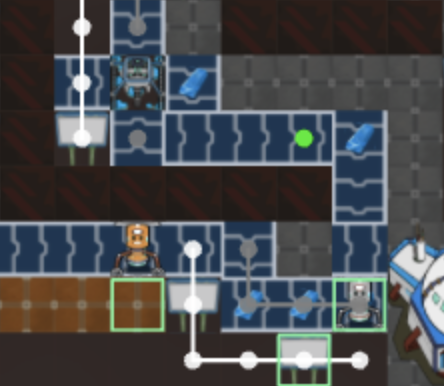
\includegraphics[width=\linewidth]{images/bfs_5.png}}
  \end{subfigure}

  \caption{Dijkstra frontier expansion over five iterations.}
  \Description{Progression of Dijkstra's algorithm, showing how the frontier expands outward from the desired target tile until we reach a tile adjacent to the builder bot.}
  \label{fig:bfs-dijkstra}
\end{figure}
\vfill\null

\begin{lstlisting}
# seed the four cost classes into the bucket
frontier[0]           = target & no_barr & no_thr
frontier[bcost]      |= target & barr    & no_thr
frontier[tcost]      |= target & no_barr & thr
frontier[bcost+tcost]|= target & barr    & thr
i = 0
while True:
    cur = frontier[i % cyc] & ~visited
    visited |= cur
    # reached a valid neighbor
    if cur & can_move_to: break
    nbr = expand_chebyshev(cur) & ~visited & ~avoid
    frontier[(i+1)    % cyc] |= nbr & nb_nt
    frontier[(i+1+bc) % cyc] |= nbr & b_nt
    ... (3 more cost classes)
    i += 1
\end{lstlisting}

When a frontier bit lands on a valid neighbor of the bot
(that is, a neighbor we can step onto right now), that direction is chosen, after a four-stage
tiebreak among reachable neighbors:

\begin{enumerate}
  \item \textbf{We prefer walkable tiles} so we don't waste our action cooldown on building a road.
  \item \textbf{We skip tiles next to borders and friendly bots} up to Chebyshev 4 if possible. Avoiding edges is good for maximizing vision. Avoiding builder bots helps prevent clumping or situations where we accidentally step onto another builder bot's target tile.
  \item \textbf{We prefer walking in zigzags.} If we walk along the same diagonal for two steps, we prefer the opposite diagonal next. The intuition is that zigzagging gives us additional vision coverage.
  \item \textbf{We prefer diagonals over cardinals}, again to maximize vision coverage.
\end{enumerate}

We also break ally barriers and place roads as needed when moving onto a tile. We will try to replace any barriers we broke at the start of each turn.

\subsection{Dijkstra's for Routing}

For routing, we define two different edge types: a conveyor step (cost 1) and a bridge step (cost 6).

When building our target tile mask, we allow for ending on existing conveyors, rather than the core itself. However, we add a cost of 4 to loaded conveyor tiles, to bias our route planner to form new conveyor lines unless the existing line is significantly better.

Since we cannot store parent pointers when running Dijkstra's, we still need to calculate the desired output of the first conveyor or bridge we should build. We do this by testing each possible output to see if it exists in the matching prior cost layer to our current tile.

We use different target tile sets when attack routing to the ring around the enemy core or routing to a foundry.

\subsection{Conveyor Cost}

We calculate the titanium cost of the optimal conveyor route to decide whether we should start building it now. This is to prevent builders from starting routes from very far away if we are low on titanium.

We calculate the cost using this formula:

\[
  \text{cost}(d)=\bigl(3\,d\,s + 0.015\,d(d-1)\bigr)\cdot 0.65,
\]


for path length $d$ at current scale $s$. This is an arithmetic series formula that lets us calculate the base $3ds$ cost of building the conveyors, with an additional $0.015d(d-1)$ term to account for the increased cost of each conveyor as scaling increases.

The $0.65$ constant is an arbitrary discount we apply to the total cost. We don't want builders to be too conservative about starting routes back to the core, since we gain titanium over time (from passive income every four turns, or other existing routes).

\subsection{BFS for Closest Target}

We used Dijkstra's for navigation and routing since we wanted to account for multiple edge weights. However, we use a much faster unweighted BFS when we want to find the closest target for action planning.

This frontier BFS mimics builder bot movement by only expanding passable tiles, minus tiles we want to avoid (such as tiles adjacent to enemy launchers). This is used when finding the closest ally building we could heal, the closest enemy we could chase, etc.

The \code{closest} function also exposes a \code{side} flag that lets us optionally run the BFS from the enemy's point of view. This is used to determine how far the enemy is from a target, which helps us reason about whether or not we could reach that target first.

\subsection{Floodfill for Voronoi Partition}

Each builder scores its states independently, so an explicit mechanism is
needed to stop builders from competing over tasks. We use a claim-partition pass that performs competing simultaneous Chebyshev flood-fills from the bot versus all other friendly bots and returns only the candidates the bot reaches first:

\begin{lstlisting}
my_front, other_front = my, others
while remaining_claims and (my_front or other_front):
    my_front    = expand(my_front)    & passable & ~claimed
    claimed |= my_front; remaining &= ~my_front
    other_front = expand(other_front) & passable & ~claimed
    claimed |= other_front; remaining &= ~other_front
return my_claimed & candidates
\end{lstlisting}

\subsection{Stuck Detection}

If more than $2 + (\text{id}\bmod 8)$ turns pass without movement progress, builder bots will move to a random adjacent tile to get unstuck. The $(\text{id}\bmod 8)$ term adds some variance based on builder bot id so that this behavior doesn't inadvertently sync up across builder bots.

\section{The Core}

The core is mainly responsible for spawning builder bots. It will also convert axionite to titanium as needed.

\subsection{Spawning Bots}

The spawn policy has multiple checks:

\begin{lstlisting}
if not has_ally and closest_enemy:
    spawn_on_core_tile_nearest(closest_enemy)
else:
    baseline = 400 if allies >= 12 else 200
    if titanium > baseline + scaling:
        spawn_toward_plan() or spawn_toward_center()
\end{lstlisting}

The first four builders are spawned in different directions for better exploration coverage at the start of the game. After that, bots are spawned toward a visible enemy if there is no ally nearby as a defensive mechanism. Otherwise, we wait until we have enough titanium and then spawn allies toward the center.

\subsection{Initial Spawn Plan}

The core orchestrates initial exploration by spawning the first four builders on the tile facing the direction they should explore.

To find the best directions, we first check which of the eight possible directions should be considered. For each direction, we check the ray pointing in that direction. If the ray's endpoint is out of vision, or there is titanium along the ray path, we consider the direction valid, since there is value in sending a builder bot in that direction.

From the set of valid directions, we pick the four that maximize the product of pairwise angular separations, to spread the directions out:
\vfill\null

\begin{lstlisting}
best = argmax over 4-subsets S of
       prod(angular_dist(a,b) for a,b in pairs(S))
\end{lstlisting}

We tiebreak by preferring diagonals if there are multiple sets of directions with the same pairwise angular separation, since diagonals give us better vision coverage.

Once we have the four initial directions, we spawn bots in order of their direction's proximity to the map center, since that is more likely to be a contested region and we want to get there before the enemy does.

\subsection{Converting Axionite}

We use the following logic for axionite conversion:

\begin{lstlisting}
if round < 1500 and titanium < 4 * harvester_cost:
    convert(clamp((3*harvester_cost - titanium)//4))
\end{lstlisting}

This allows us to convert axionite to titanium when we are running low, up until turn 1500, since accumulating axionite for the tiebreaker is important in long-running games that might reach round 2000.

\section{Builder Bots}

Builder bots do the following each turn:

\begin{enumerate}
  \item \textbf{Update map info} using the cambc controller and any learned map info from ally markers
  \item \textbf{Rebuild broken barriers} if we destroyed any previously for movement
  \item \textbf{Score states} and run the best state
  \item \textbf{Place a launcher or barrier} if we detect a nearby chokepoint
  \item \textbf{Heal an adjacent building} and fall back to healing ourselves otherwise
  \item \textbf{Destroy enemy feeders} if adjacent
  \item \textbf{Try spamming roads} if empty tile adjacent
  \item \textbf{Place marker} to broadcast symmetry and map info
\end{enumerate}

An enemy feeder is an ally conveyor, bridge, or harvester that outputs onto an enemy turret. For harvesters, we also check that there are no ally turrets before destroying it.

When spamming roads, we prioritize placing roads adjacent to ally conveyors. We also place roads around enemy bots or buildings if an enemy is nearby. Road spam helps us with map control since enemies have to destroy the roads first before they place their own buildings. We do not spam roads in front of our gunners to keep their firing path unblocked.


\subsection*{Persistent Builder State}

There are a few exceptions to our memoryless architecture. We maintain TTL caches for each state so that builders will not reconsider target tiles that failed recently. We also change the behavior of the first few builders:

The very first builder spawned will restrict its targets to squared distance $\leq 100$ of the core, so it stays near the core as a guard.

The first four builders will check the tile they spawn on to decide their initial explore direction (see \hyperref[sec:initial-explore]{Initial Exploration}). They will clear this target upon arrival or after a $30$-round timeout.

\section{States}

Builder bots have seven possible states they can run. Every state exposes a \code{score()} function that uses global map info to calculate state priority and return a value strictly below a fixed ceiling (shown in Table~\ref{tab:states}). We then run the logic for the highest scoring state.

\begin{table}[htbp]
  \caption{Builder states by score ceiling.}
  \label{tab:states}
  \begin{tabular}{llp{0.45\linewidth}}
    \toprule
    State   & Max  & Role                    \\
    \midrule
    attack  & 9    & build sentinel / gunner \\
    heal    & 8    & repair / chase invaders \\
    route   & 7.75 & route resources back    \\
    secure  & 7.5  & surround an ore tile    \\
    harvest & 4    & build a harvester       \\
    disrupt & 2    & barrier enemy-side ore  \\
    explore & 1    & explore unseen tiles    \\
    \bottomrule
  \end{tabular}
\end{table}

We calculate state scores in descending order of the max possible score for that state. This avoids having to compute \code{score()} on lower-ceiling states that cannot win once we've found a provably better score:

\begin{lstlisting}
for state in states_desc:        # sorted by MAX_SCORE
    if best_score >= state.MAX_SCORE:
        break
    s = state.score()
    if s > best_score:
        best_score, best = s, state
\end{lstlisting}

\subsection{State Pattern}

Each state follows the same pattern. The \code{score()} function derives candidate tiles for the state (such as buildings we can heal for heal state). We intersect the candidate tile set with a Voronoi claim partition to avoid multiple builders contesting the same target tile. We then cache the result for \code{run()} to use if the state ends up being chosen.

\subsection{Attack (ceiling 9)}

Attack is our highest priority state where we place turrets to target enemy buildings. We prefer placing turrets on empty tiles or less important infrastructure (roads, guard conveyors, etc). We will fall back to placing on non-guard conveyors/bridges or enemy infrastructure we could damage, but at a higher threshold.


\statefigure{images/attack.png}{Attack.}{}

\subsection{Bit-Sliced Score Planes}

For each facing and turret type, we maintain a score plane stack: a list of $9$ bitmasks where bit $i$ of the integer score at tile $n$ is \code{(planes[i] >> n) \& 1}. This lets us do bulk score updates and queries over the whole board with bitwise parallelism, rather than iterating over an array.

To add a constant $c$ to the score of every tile in a mask $M$, for each set bit of $c$ we XOR the corresponding plane with $M$ (toggling that digit at every tile in $M$ simultaneously) and ripple any AND-carries up through higher planes:

\begin{figure*}[t]
  \begin{lstlisting}
# Add the constant c (c = sum of 2^b for b in `bits`) to the stored score of EVERY tile in `mask`,
# in O(NUM_PLANES) whole-board big-integer ops -- cost independent of how many tiles are in `mask`.
def add_bits_to_planes(planes, bits, mask):
    for i in bits:                          # for each set binary digit of the constant c
        carry = planes[i] & mask            # tiles where digit i overflows
        planes[i] ^= mask                   # add c's i-th digit to all those tiles at once
        j = i + 1
        while carry and j < NUM_PLANES:     # ripple the carry up through higher planes
            new_carry = planes[j] & carry
            planes[j] ^= carry
            carry = new_carry; j += 1

# Bitmask of tiles in `cands` whose stored score >= thr, computed in one MSB-first pass.
def ge_threshold_mask(planes, thr, cands):
    eq, gt = cands, 0
    for i in range(NUM_PLANES - 1, -1, -1):
        p = planes[i]
        if (thr >> i) & 1: eq &= p          # thr digit set: tile must match to stay "equal so far"
        else: gt |= eq & p; eq &= ~p        # thr digit clear: a set score digit => strictly greater
    return gt | eq
\end{lstlisting}
  \caption{The two main bit-sliced primitives. \code{add\_bits\_to\_planes} adds a score constant
    to an arbitrary set of tiles in $O(\text{planes})$ big-integer operations regardless of how many tiles
    are in the set. \code{ge\_threshold\_mask} thresholds the whole board against a scalar in one pass from
    the most significant bit down.}
  \Description{Python code listing showing two functions: add_bits_to_planes, which adds a constant to the stored score of every tile in a mask using O(NUM_PLANES) big-integer operations independent of the mask's tile count; and ge_threshold_mask, which returns a bitmask of tiles whose stored score is at least a given threshold in one MSB-first pass over the planes.}
  \label{lst:planes}
\end{figure*}

The key property is that the cost of calculating scores is independent of the number of tiles scored. The per-digit loop is bounded by the fixed plane count, and each iteration is one big-integer AND/XOR over the whole map. This is what makes exhaustive placement evaluation fit within our per-turn budget.

\subsection{Scoring Tiles}

We group enemy building types by equal score so one masked add handles a whole score class. For each of the eight facings, the sentinel pass shifts each enemy-type mask by the reverse of every sentinel attack offset under that facing and ANDs with the valid-placement mask. Wherever a bit survives is a tile from which a sentinel facing $d$ would hit that enemy, so we add the type's score into the planes there.

The advantage of this approach is that we never iterate over individual placement tiles. The total time scales with the number of hit offsets, facings, building types, and score bits, rather than with the board size.

Gunner scoring follows the same idea along a directional ray of up to three steps. The score is discounted by $0.9^k$ at step $k$, the ray is blocked by walls and our own non-road buildings, and the core is single-counted at its closest hit. This step discount prioritizes placing gunners directly adjacent to targets, since they can't shoot over tiles like sentinels can. We also add a rotation bonus equal to the sum over all eight facings shifted right by 3, to still favor targets we might rotate toward later.

We apply a penalty to placement positions under threat by enemy turrets. We also apply a penalty to placements that would destroy an ally non-guard conveyor or bridge. All of this is memoized per round keyed by the structural state, enemy presence, and placement masks.

\subsection{Filtering Tiles}

The candidate pass returns the legal placement mask per facing direction. We seed from tiles fed by titanium or axionite, plus the Manhattan dilation of titanium harvesters and foundries not already used by one of our sentinels. Sentinels consume more ammo than a harvester can provide, so we avoid building multiple around the same harvester.

We then intersect with seen and buildable tiles, and remove:

\begin{itemize}[leftmargin=*]
  \item Tiles within a two-step enemy-bot BFS through their passable graph. We treat our launcher 3x3 zones as impassable for enemies, since an enemy entering one is flung back.
  \item Our own turret feed chains, so a new placement never cuts off an existing turret.
  \item Per-direction loader blockers, since feeders cannot load a turret pointing into them.
\end{itemize}

Sentinels additionally exclude tiles within enemy gunner or breach range, since they shoot slowly and are unlikely to win the trade. Gunners are permitted on those tiles to enable harvester combat.

We only consider placement tiles whose scores pass a threshold. Sentinels and gunners have different thresholds, since they have slightly different scoring systems. The threshold is also higher for enemy infrastructure we would have to destroy first before placing, or ally infrastructure we don't want to destroy (non-guard conveyors and bridges).
\statefigure{images/attack_candidates.png}{Valid turret locations. Gunner in red and sentinel in blue.}{fig:attack_candidates}
\subsection{Placing Turrets}

If we can place a turret on a preferred tile this turn, either from our current tile or an adjacent tile, we pick the highest scoring such placement. This is to favor turrets we can place this round over potentially better placements we would only reach in a later round.

Otherwise, we pick the closest preferred or fallback tile. Among candidates within two BFS steps, we maximize
\[
  \text{enemyBFS}_{\text{adj}}(\text{cand}) - \text{myBFS}(\text{cand}),
\]
treating our launcher zones and barriers as enemy-impassable.

If the target is an enemy conveyor that a visible enemy could heal, we scan adjacent buildable tiles for a launcher or barrier placement that strictly increases the enemy's BFS distance to the conveyor without worsening our own approach. Barriers require a delta of at least 2; launchers require at least 5, reflecting their relative cost.

\statefigure{images/anti_chase.png}{This launcher prevents the enemy from advancing, as the launcher's 3x3 and the barrier form a wall}{}

We normally avoid damaging enemy conveyor targets if a nearby enemy could heal them. However, we have three exceptions:

\begin{itemize}[leftmargin=*]
  \item We locally outnumber the threat (at least 2 ally builder bots within squared distance 25 versus a single enemy within two BFS steps).
  \item An allied sentinel is in sight, so we damage more than they can heal anyway.
  \item The target's 3x3 is fully sealed by walls, non-walkable buildings, or our launcher 3x3s, so enemies cannot reach the target tile.
\end{itemize}

\subsection{Heal (ceiling 8)}

The heal state defends against opponent attacks in two ways. First, we heal damaged ally buildings adjacent to us. Second, we chase enemy bots that wander into our conveyor zone before they can attack our infrastructure.

Score returns 7 if any friendly building has more than 2 damage, or if a friendly sentinel and enemy sentinel are within each other's attack ranges. We treat these sentinels as very damaged so we stay near it as they trade damage with the enemy sentinel. Score also returns 7 if a chase target exists within the conveyor zone, defined as within 8 pathing steps of a conveyor. We score 2.5 if a chase target exists but is farther.

\statefigure{images/heal.png}{Heal.}{}

At the end of each turn, we scan adjacent tiles and heal the one maximizing damage times a fixed type priority. We consider all very damaged buildings before less damaged ones, and consider six priority tiers:

\begin{enumerate}
  \item Core
  \item Turrets
  \item Armored conveyors, harvesters, and foundries
  \item Regular conveyors
  \item Barriers, bridges, and splitters
  \item Roads
\end{enumerate}

For chase target selection, we remove enemies under attack by a turret and enemies that another friendly bot is strictly closer to. We then prefer the closest surviving target.

When chase fails on pathing, the launcher fallback fires as a counter-launcher response:

\begin{lstlisting}
for enemy on a damaged friendly conv (unclaimed):
  # T1: placeable cell adjacent to enemy
  T1 = adj(enemy) of those four types
  # T0: a stand-tile within 8 BFS steps of T1
  T0 = adj(T1) reachable within 8
  pick (enemy, T1) minimizing my dist to T0
\end{lstlisting}


This most commonly happens when an enemy places a launcher to keep our bot away from its attack target. In this case, we place a launcher in response to keep their bot away. We will place a gunner instead if the target tile is one of our guard conveyors.

\subsection{Route (ceiling 7.75)}

The route state builds conveyor lines from harvesters back to the core. It tries to route from dead-end conveyors, orphan harvesters, and orphan foundries. A structure is an orphan if it hasn't been routed back yet and has at least one cardinal neighbor we can build on.

Score returns 5 normally, but 7.75 (above heal's 7) when any claim is important:

\begin{lstlisting}
important = expand_chebyshev(enemy_bots, 5)
            & ~(my_harvesters | my_foundries)
            | feeding_enemy
return 7.75 if important & claims else (5 if claims else 0)
\end{lstlisting}

We will place armoured conveyors instead of normal conveyors if we have axionite available and at least $5\times$ the cost in titanium.

If we don't have enough to continue routing, but there is an enemy nearby, we place a barrier on the dead-end's output, or the dead-end conveyor itself if needed, to prevent enemies from taking advantage of it.

When placing conveyors, we upgrade to armored conveyors when we have at least 5x their cost in titanium and we have axionite available.

\subsection{Attack Route (override)}

We added attack routing in Khaos for the final tournament. Instead of routing resources back to our core, the builder extends the conveyor network toward the opponent to disrupt their economy and infrastructure. The override triggers when our BFS distance to the enemy core is at most $1.5\times$ our BFS distance to our own core.

In testing, we found that aggressive attack routing was usually a net win. Even when the route never reached the enemy core, the damage it caused to enemy infrastructure and area control was usually enough to justify the loss of resources.

\statefigure{images/attack_route_1.png}{Attack Route.}{}

If we realize we can extend the route into a gunner, we do that instead. We only place a sentinel when a gunner would be significantly worse, such as when we need to shoot enemy buildings from behind a wall.

\statefigure{images/attack_route_2.png}{Attack Route with Gunner.}{fig:state-attack-route-gunner}

In Figure~\ref{fig:state-attack-route-gunner}, rather than simply placing a sentinel to shoot the core, in two out of the three routes, the bot realized that the route could be extended slightly to support a gunner. In the third route, enemy roads blocked the extension, so it opted for a sentinel instead.

\subsection{Secure (ceiling 7.5)}

Secure and harvest generally execute in sequence. Secure first places guard conveyors on the four cardinal neighbors of an ore tile. Once the tile is secured, harvest places a harvester on it. This sequence prevents enemies from placing turrets to take advantage of harvesters with exposed sides.

\statefigure{images/secure.png}{Secure.}{}

The secure state scores 7.5 if a claim sits on an already-built harvester or foundry, since we don't want to leave these buildings exposed to enemy turret placements. The state scores 3 if there is an ore, but no harvester yet, since we still want to secure it before we harvest.

We generally secure an ore using guard conveyors. These inward-facing conveyors are not valid outputs of the ore tile, so they never actually carry resources. However, they prevent the enemy from placing a turret adjacent to the ore, and they have significantly more health than a road. We place these instead of barriers to improve the traversability of our infrastructure for builder bots.

While securing, we also compute the optimal route and place the first conveyor facing outward, instead of guarding by facing inward, to slightly speed up our economy.

The route-target pass detects this pattern via a guard-conveyor mask so that conveyors whose target is open ore are excluded from the routing graph.

To prevent oscillations that would otherwise occur as the builder bot moves to place guard conveyors, when it is close enough to several unsecured ores, it will pick the most secured ore (the most sides covered) within Chebyshev distance 2, rather than just the closest one.

\subsection{Harvest (ceiling 4)}

Harvest places a harvester on an ore tile. We pick from possible ore tiles that don't already have a harvester and are secured.

The possible-ore mask includes titanium ore, plus axionite ore after round 750 if we've already harvested titanium. It excludes landlocked ore (ore whose four cardinal neighbors are all ore or unseen, since these are difficult to reach by conveyor). We also avoid existing ally infrastructure (conveyors, bridges, etc.), enemy blocking buildings, and tiles under enemy turret threat.

\statefigure{images/harvest.png}{Harvest.}{}

We compute \code{secured()} for the entire map using bitmask operations. A tile is secured if every cardinal side is off the map, a wall, or one of our non-road non-marker buildings.

If building the conveyor line to the target is too expensive, we add the tile to a temporary failure cache so we don't consider it for 100 rounds.

\subsection{Disrupt (ceiling 2)}

Disrupt places barriers on ore tiles outside our harvest zone, to block the enemy from harvesting them. We skip ores under enemy turret or launcher coverage. This state only runs when we have significant resources (at least five harvesters worth of titanium), and acts as a cheap way of denying the enemy's economy.

If the target tile already has an enemy road, we fire on it first. If it's a friendly road or marker, we destroy it and then place a barrier.

\statefigure{images/disrupt.png}{Disrupt.}{}

\subsection{Explore (ceiling 1)}

If we have nothing better to do, our builder bots wander toward unexplored territory.

Our first few bots have their own initial explore logic. Otherwise, we wander toward a random tile near the frontier of our explored region.

\subsection*{Initial Exploration}
\label{sec:initial-explore}

For the first four builders, the core uses the tile it spawns each builder on to communicate which direction the builder should explore. This lets the core orchestrate initial exploration for better coverage.

On the new builder's first turn, it reads its own position relative to the core, recovers the intended facing by comparing its tile with the core, and reproduces the same ray-endpoint computation the core runs, capped at 12 Chebyshev steps to prevent the bot from wandering off too far.

The bot follows that target until it is within squared distance 18 or 30 rounds have elapsed, after which the slot is cleared and default explore takes over.

\subsubsection*{Frontier Sampling}

If not following the initial explore plan, the explore-target generator floodfills from the bot's current position and other known friendly bot locations. It then samples a random tile from a frontier ring near the edge of the explored area once the flood terminates:

\begin{lstlisting}
seeds = me | friendly_bots
frontier = seeds; ring_buffer = deque(maxlen=6)
while frontier and c < 100:
    frontier = expand_chebyshev(frontier) & passable
               & ~visited
    visited |= frontier; ring_buffer.append(frontier); c+=1
target = random_bit(ring_buffer[0])     # the ring at c-5
\end{lstlisting}

Seeding from teammates biases each bot's frontier away from where
others already are, allowing for better area coverage.

\section{Turrets}

Sentinels and gunners share the same priority system for scoring tiles. The goal is to prioritize disrupting the enemy infrastructure as much as possible, by considering in order:

\begin{enumerate}
  \item Enemy foundries that feed at least one enemy turret and none of mine.
  \item Enemy harvesters that feed more than one enemy turret and none of mine.
  \item Enemy turrets that can hit one of my turrets, plus the enemy conveyors that feed them and the harvesters whose chain reaches them.
  \item As (3) but for any enemy turret, dropping the ``threatens mine'' guard.
  \item Enemy builder bots
  \item Enemy roads, conveyors, splitters, bridges, or barriers cardinally adjacent to any harvester on either team.
  \item Any enemy entity, other than roads or markers
\end{enumerate}

If any target is adjacent to two or more enemy builder bots, we consider it after all of the priorities above, regardless of its normal priority.

Within each priority, we tiebreak by considering:

\begin{enumerate}
  \item The highest health entity we could one-shot
  \item The entity furthest from enemy builder bots (so it takes them longer to move toward and heal it)
  \item The highest weight entity (varies between gunner and sentinel, but generally prefers shooting enemy turrets, then infrastructure)
  \item The lowest health entity
\end{enumerate}

We ignore conveyors, harvesters, or foundries that feed our own turrets, so we don't shoot enemy buildings that we are benefiting from. We also ignore buildings if an ally builder bot is on the same tile, since the builder bot would be hit instead.

\subsection{Sentinel}

Our sentinels coordinate shots by waiting to shoot if they notice an ally sentinel recently shot a target in vision. This applies if we see a target's health drop and see another ally sentinel with that target also in vision. In this case, we wait until the health drops again so we can shoot on the same turn and destroy it before enemy builder bots can heal.


\begin{lstlisting}
if locked and can_one_shot(locked):
    fire(locked)
elif locked:
    wait    # don't waste 18 dmg
elif select_best gives a one-shot:
    fire it # one-shots ignore lock
else:
    fire select_best pick
\end{lstlisting}

We only coordinate one-taps this way for sentinels with a higher id than the other ally sentinel in vision. This is because entities act in increasing id order, so the higher-id sentinel will always be able to react to the lower-id sentinel's shot within the same turn, but not vice versa.

Our sentinels will consider self-destructing if they are not adjacent to a harvester and there is no enemy builder bot nearby. They will self-destruct after 16 turns if they have no ammo, or after only 4 turns if they also have no possible upstream feeder.


\subsection{Gunner}

Gunners can only shoot in their facing direction, so we fire if there is an enemy target in front of us. Otherwise, we consider rotating if we see an enemy building, or an enemy bot standing on a damaged ally conveyor that doesn't have a nearby ally builder bot to heal it. This is to prevent enemies from continuing to freely attack the conveyor.

Rotation requires at least 60 global titanium, so a gunner doesn't burn our economy by rotating repeatedly.

\subsection{Launcher}

Launchers throw enemy bots. A launcher classifies itself once on placement. A chokepoint launcher (one with no enemy conveyor within its $3\times3$) first tries to fling the enemy back to a tile they recently occupied, using the tracked per-bot position history. This forces them to retrace their path.

If that fails, or for offensive and defensive launchers, we use the region-minimizing throw heuristic. For every legal destination, we Chebyshev-flood the region the bot could navigate from there, using enemy-POV passability and treating unseen tiles as impassable. We then choose the destination that yields the smallest reachable region. We tiebreak by greatest wall-only BFS distance from the seed set consisting of every conveyor plus the launcher itself:

\begin{lstlisting}
for dest in legal_launch_tiles:
    region = flood_chebyshev(dest, enemy_passable
                             & seen)
    size[dest] = popcount(region)
throw to argmin (size[dest], -wall_bfs_dist(dest))
\end{lstlisting}

The effect is to either keep the enemy out of our territory, or keep them away from a tile we are trying to disrupt.


\section{Chokepoint Detection}

We also have a significant amount of logic geared around chokepoint
detection and subsequent launcher or barrier placement, and so will dedicate the next few pages to that. Chokepoint
detection starts running once we have learned enough of the map, and then
continues running in the background through an incremental save-state for
the rest of the game.

The goal is to produce a small set of tactically useful tiles where a single
barrier or launcher can change the connectivity of the map. In practice,
these are narrow corridors between larger regions, especially corridors
that separate our controlled territory from the opponent's side. Due to
features such as barrier walkthrough and a launcher effectively blocking a
$3\times3$ area, these regions become chokepoints that only our bots can pass.

\begin{figure}[htbp]
  \centering
  \begin{minipage}{0.32\linewidth}
    \centering
    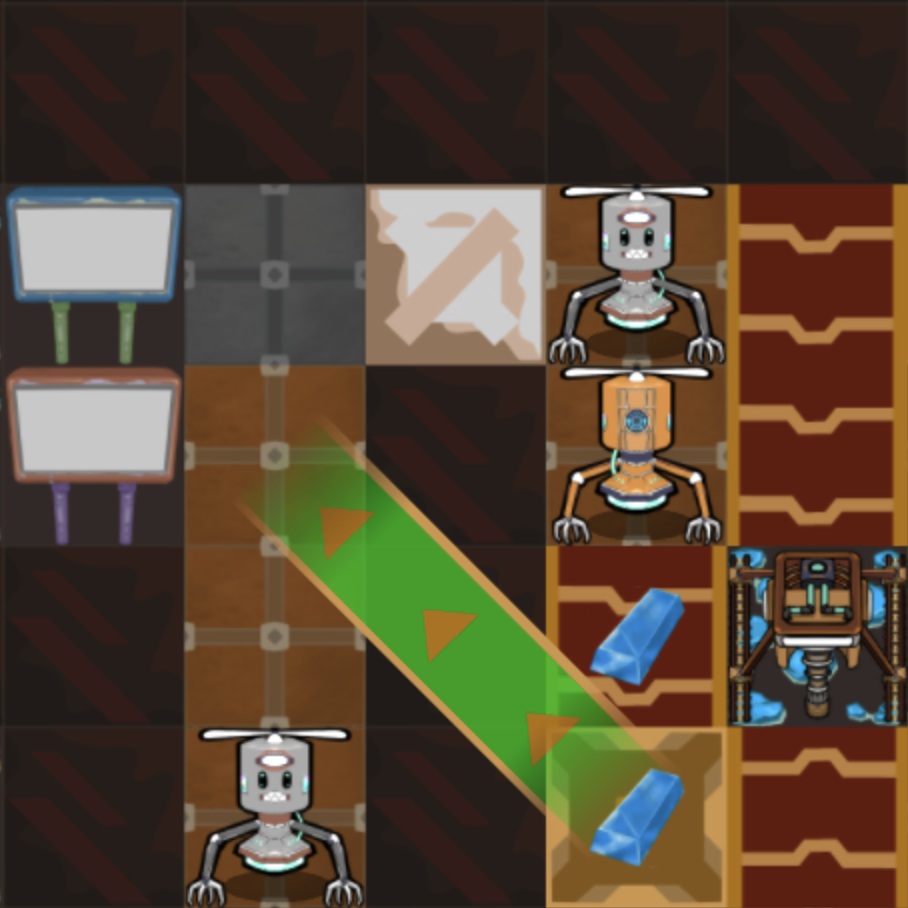
\includegraphics[width=\linewidth]{images/walkthrough_1.png}\\
  \end{minipage}
  \hfill
  \begin{minipage}{0.32\linewidth}
    \centering
    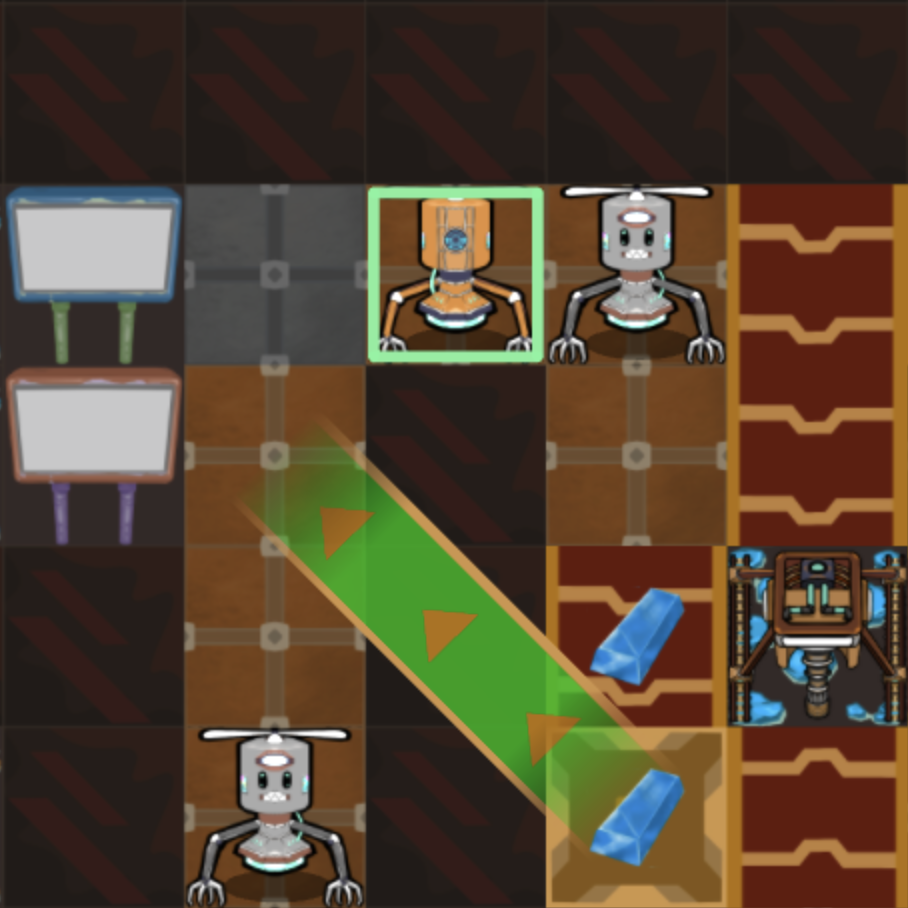
\includegraphics[width=\linewidth]{images/walkthrough_2.png}\\
  \end{minipage}
  \hfill
  \begin{minipage}{0.32\linewidth}
    \centering
    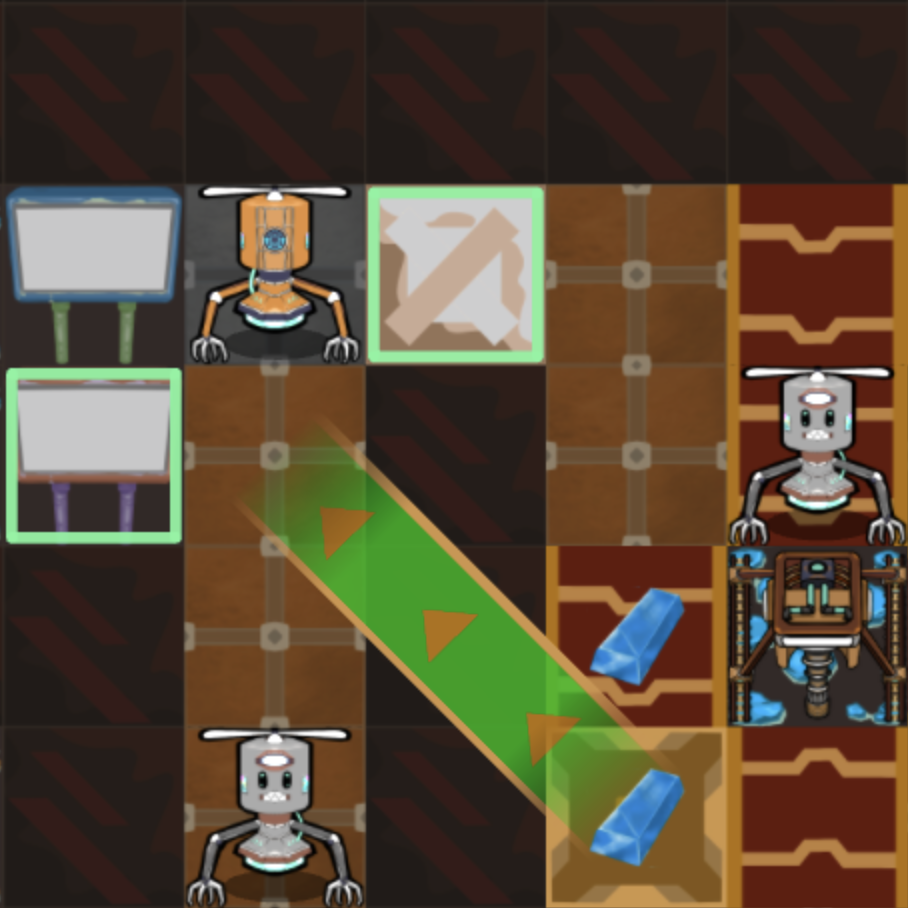
\includegraphics[width=\linewidth]{images/walkthrough_3.png}\\
  \end{minipage}
  \caption{Chokepoint barrier walkthrough.}
  \Description{Three side-by-side game screenshots showing a chokepoint barrier walkthrough: ``Approach'' shows a builder moving toward an existing barrier, ``Destroy'' shows the builder breaking through it, and ``Barrier'' shows a fresh barrier placed behind the builder to re-seal the chokepoint.}
\end{figure}



\subsection{Simplified Geometry Core}
The standalone chokepoint logic needed to run without SciPy,
Shapely, NumPy, or compiled geometry libraries since they were banned for this competition. Hence, a custom
geometry engine was needed. The base library was vendored from the \href{https://github.com/Yatoom/foronoi}{Foronoi Python library}, but completely restructured and optimized for the purposes of this competition.

The core idea was to replace heavyweight polygon operations with a small
raster-backed geometry layer. The map is first lifted into a higher-resolution boolean mask, where each game tile becomes a small
\code{scale}\,$\times$\,\code{scale} block. The scale is derived from the
requested sample spacing, giving enough sub-tile precision for geometry
while keeping the whole map tiny:

\begin{lstlisting}
scale = raster_scale_from_spacing(sample_spacing)

analysis_mask = build_analysis_mask(rows, cols, scale,
                                    analysis_polygon)
obstacle_mask = build_obstacle_mask(walls, rows, cols,
                                    scale, analysis_mask)

kept_obstacles, discarded = split_obstacle_mask_by_area(
    obstacle_mask, min_area * scale * scale)

free_mask = build_free_mask(analysis_mask, kept_obstacles)
\end{lstlisting}

The old version relied on polygon union, difference, intersection, and
boundary extraction from external libraries. The runtime version instead
does each step directly on the mask: scanline polygon fill for the analysis
region, block filling for wall tiles, flood-fill component filtering for
small discarded obstacles, and boolean subtraction for free space. Since
the maps are at most $50\times50$, even a moderately upsampled mask is
small enough for pure Python.

Once free space is known, the boundary is extracted by scanning for
free/non-free transitions. Consecutive collinear boundary pixels are merged
into longer axis-aligned segments, which keeps the later sampling step much
smaller than treating every raster edge independently:

\begin{lstlisting}
segments = boundary_segments_from_mask(free_mask, scale)

# Internally:
# - scan top/bottom exposed edges row-wise
# - scan left/right exposed edges column-wise
# - merge adjacent horizontal and vertical runs
\end{lstlisting}

Those merged boundary segments become the input sites for a sweep-line Voronoi implementation. In float mode, the runtime
chokepointer sets the numeric backend to ordinary Python floats rather
than \code{Decimal}. This loses arbitrary precision, but the inputs are
already quantized to map/sub-tile coordinates, and the speedup is large
enough to matter for all-map iteration.
\vfill\null

\begin{lstlisting}
set_foronoi_numeric_mode("float")

points = collect_boundary_samples(sample_spacing)
vor = Voronoi(Polygon(analysis_polygon))
vor.create_diagram(points=points)

for edge in vor.edges:
    p1 = edge.origin()
    p2 = edge.twin.origin()
    if segment_is_inside_free_space(p1, p2):
        add_raw_edge(p1, p2)
\end{lstlisting}

The runtime also replaces geometric containment queries with mask
containment. A candidate Voronoi edge is accepted only if several sampled
points along the segment remain inside the free-space mask:

\begin{lstlisting}
def segment_is_inside_free_space(a, b):
    steps = max(5, ceil(length(a,b) * scale * 2))
    for k in range(1, steps):
        p = lerp(a, b, k / steps)
        if not point_is_inside_free_space(p):
            return False
    return True
\end{lstlisting}

Finally, each Voronoi vertex needs a clearance radius, which is the
distance to the nearest wall/free-space boundary. Instead of asking a
geometry library for distance-to-boundary, the runtime stores the merged
boundary segments in two flat lists: vertical segments and horizontal
segments. Radius then becomes a direct minimum over squared point-to-segment
distances:

\begin{lstlisting}
best = INF

for x0, y1, y2 in vertical_boundaries:
    dx = x - x0
    dy = clamp_distance_to_interval(y, y1, y2)
    best = min(best, dx*dx + dy*dy)

for y0, x1, x2 in horizontal_boundaries:
    dy = y - y0
    dx = clamp_distance_to_interval(x, x1, x2)
    best = min(best, dx*dx + dy*dy)

radius = sqrt(best)
\end{lstlisting}

This float runtime is intentionally less general than a full geometry
kernel. It only needs axis-aligned tile maps, clipped analysis polygons,
boundary sampling, free-space containment, and clearance radii. By
specializing to exactly those operations, the chokepointer stays fully
pure Python and remains fast enough to run.

\subsection{Online Save-Stating}
This separation was important. The geometry code is relatively complex,
whereas the in-game usage has to be simple and robust. The builder should
not care whether a chokepoint came from a Voronoi edge, a pruned graph
chain, or a merged region boundary. It only needs to know whether standing
near a tile and spending an action there is likely to improve our position.

At a high level, the pipeline is:

\begin{lstlisting}
known_walls = map_info.wall_mask_from_seen_and_symmetry()

state = chokepoint_state.resume_or_init(known_walls)
state.step_until_budget()

if state.finished:
    for choke in state.blocker_candidates:
        register_chokepoint_tile(choke.tile,
                                  choke.kind,
                                  choke.radius)
\end{lstlisting}

The actual computation is too expensive to run from scratch inside a
single builder turn, so the analyzer is incremental. Each call performs a
bounded amount of work and stores the intermediate state globally. Once it
finishes, the resulting chokepoint tiles are cached until the known wall
map changes enough to invalidate them. This is why our builder bots time out every turn.

\subsection{Map Reduction}

The first step is to decide which part of the map we actually need to
analyze. Because every map is symmetric, once symmetry is solved we only
analyze our half of the map and mirror the result. This cuts the work by
roughly a factor of two and also prevents duplicate chokepoints from being
reported on both sides of the same symmetric corridor.

\begin{lstlisting}
if symmetry == VERTICAL:
    analysis_poly = half_map_containing(my_core)
elif symmetry == HORIZONTAL:
    analysis_poly = half_map_containing(my_core)
elif symmetry == ROTATIONAL:
    analysis_poly = clipped_by_perpendicular_bisector(
        my_core, enemy_core)
else:
    analysis_poly = full_map
\end{lstlisting}

The input to the geometric pipeline is the set of known walls intersected
with this analysis polygon. Unknown tiles are treated conservatively: we do
not want to plan a permanent blocker around a corridor that may later turn
out not to exist. Symmetry broadcasts help here because they let us infer
far-away walls before physically exploring them.


\subsection{Voronoi Skeleton}

The main version of the detector uses a Broodwar Terrain Analyzer (BWTA)-adjacent medial-axis
approximation. We sample points along the boundary of the free space:
outer map boundary, wall perimeters, and any obstacle holes. Then we run a
Voronoi diagram over those samples. Voronoi edges that lie inside free
space approximate the medial axis of the traversable map.

\statefigure{images/voronoi.png}{Voronoi on "Cubes"}{}

The intuition is that a point on this graph is equally far from two or
more obstacle boundaries. Wide open rooms produce high-radius graph
regions, while narrow corridors produce low-radius graph chains between
those regions.

\begin{lstlisting}
samples = []
for segment in free_space_boundary:
    samples.extend(sample_segment(segment, spacing=1.0))

diagram = voronoi(samples)

for edge in diagram.edges:
    if edge.is_finite() and edge_inside_free_space(edge):
        graph.add(edge)
\end{lstlisting}

For each graph vertex, we compute a clearance radius: the distance from
that vertex to the nearest free-space boundary. This radius is the main
scalar used by the later pruning and chokepoint extraction passes.

\begin{lstlisting}
for v in graph.vertices:
    radius[v] = distance(v, free_space.boundary)
\end{lstlisting}

A small radius means the vertex lies in a tight corridor. A large radius
means the vertex lies in an open area. Chokepoints are not simply the
smallest-radius vertices, because wall corners and dead-end branches also
have tiny radius. They are the smallest-radius vertices on meaningful
paths between larger regions.

\subsection{Graph Pruning}

The raw Voronoi graph contains many branches that point into wall corners
or small pockets. These are not useful chokepoints, because blocking them
does not separate two important regions. We prune these branches with a
simple radius monotonicity rule.

Leaves are removed if they are narrower than their parent. Repeating this
peels off branches that run from open space into a dead end or wall
corner, while preserving chains that connect two larger areas.

\begin{lstlisting}
active = all_vertices
queue = leaves(graph)

while queue:
    leaf = queue.pop()
    parent = only_neighbor(leaf)

    if radius[leaf] < radius[parent]:
        remove leaf from graph
        if degree(parent) == 1:
            queue.push(parent)
\end{lstlisting}

\begin{figure}[htbp]
  \centering
  \begin{minipage}{0.42\linewidth}
    \centering
    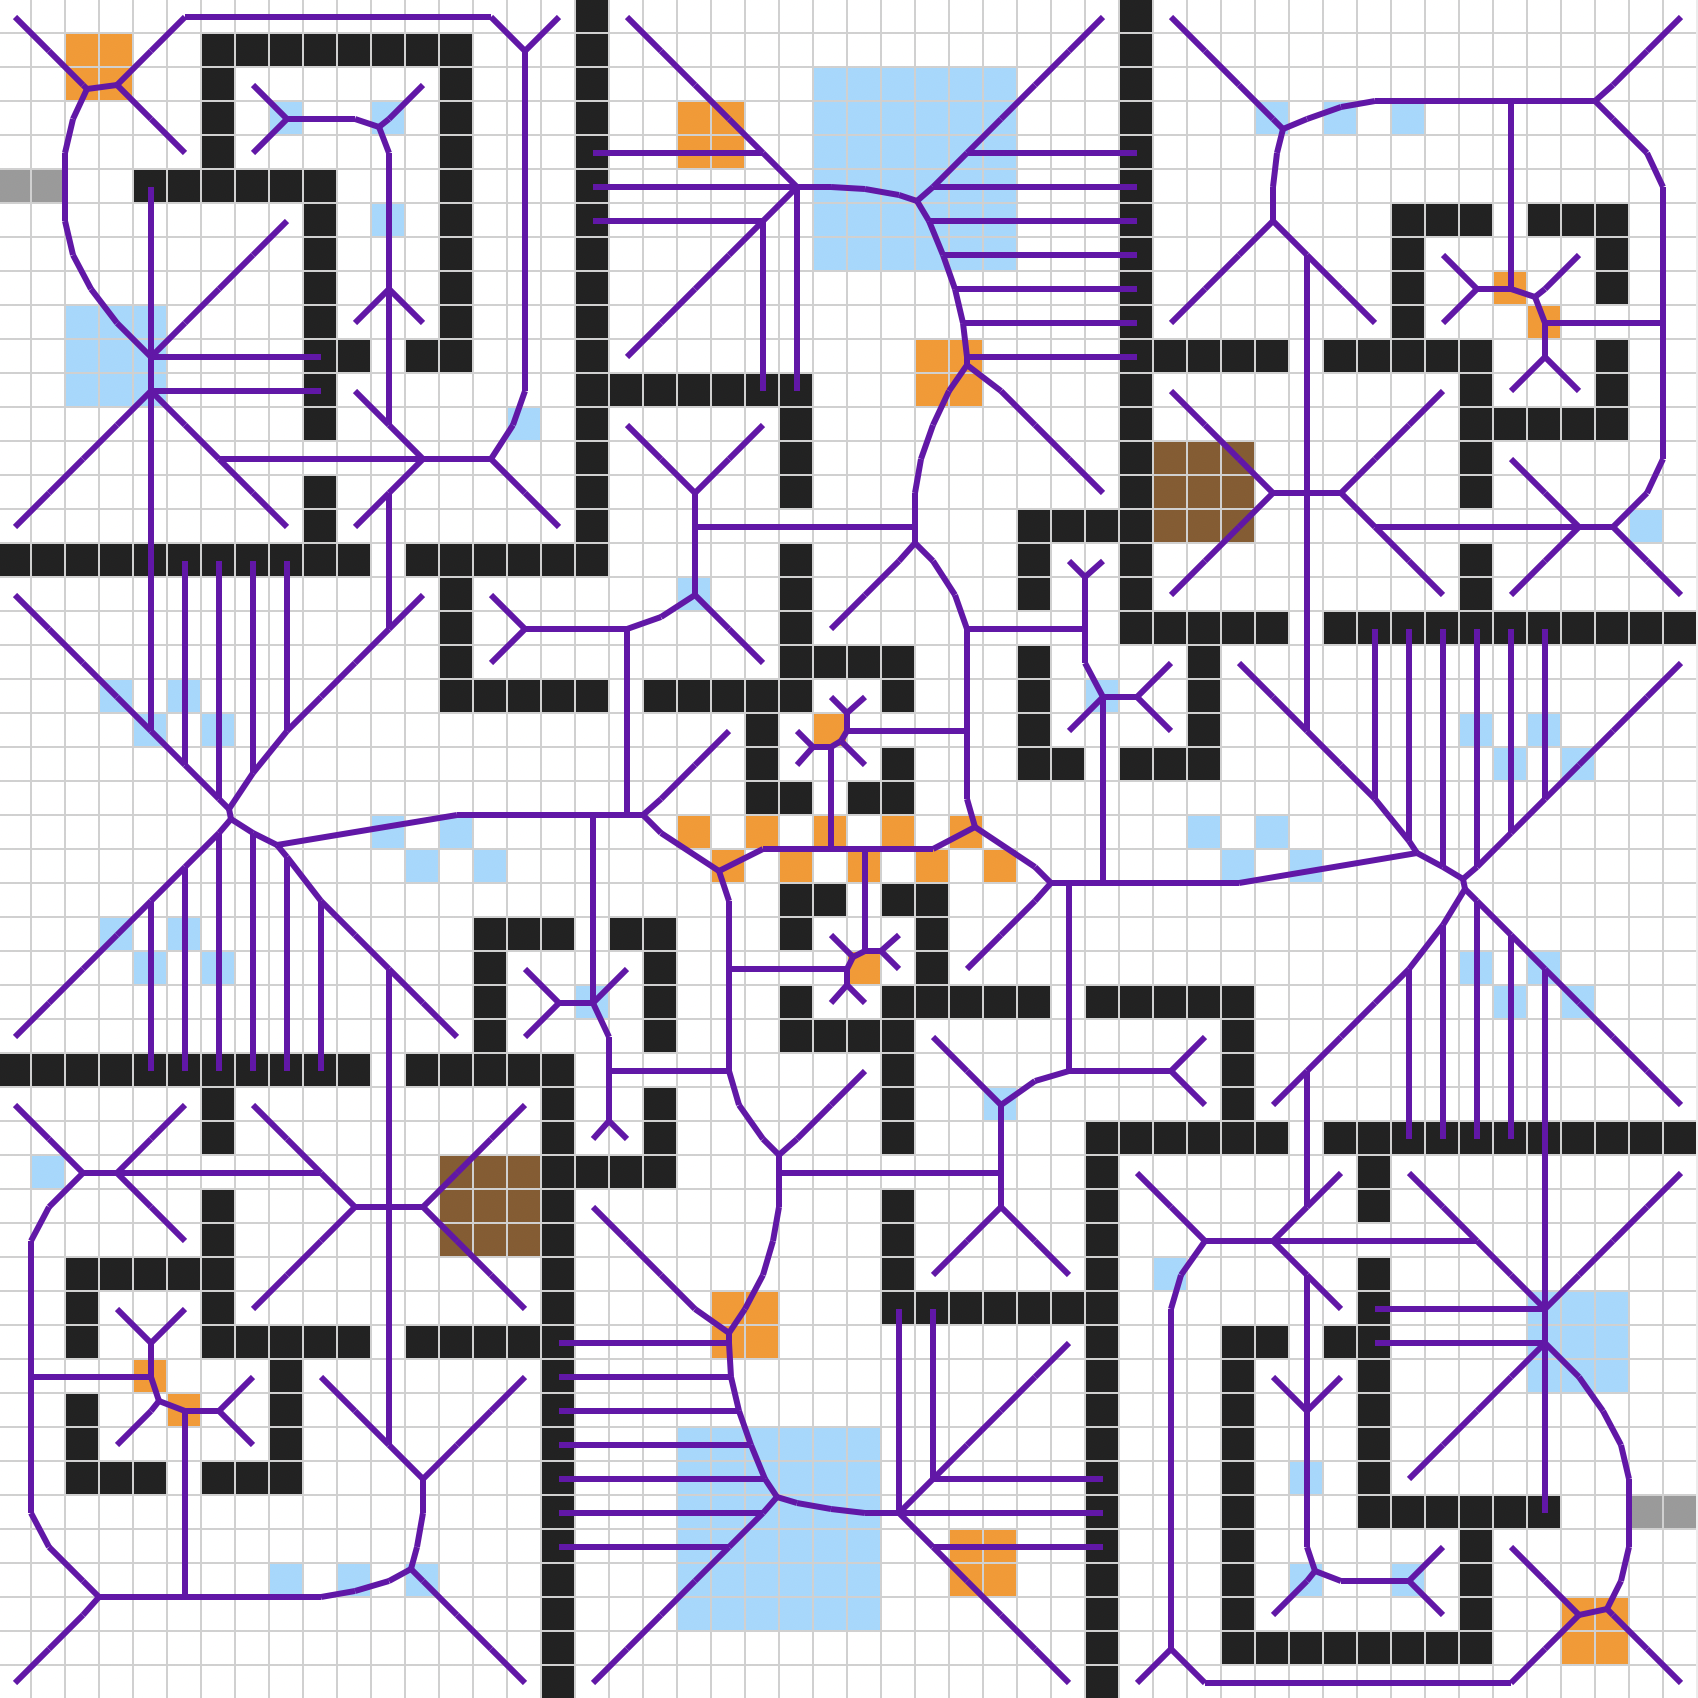
\includegraphics[width=\linewidth]{images/voronoi.png}\\
    {\small Unpruned}
  \end{minipage}
  \hfill
  \begin{minipage}{0.42\linewidth}
    \centering
    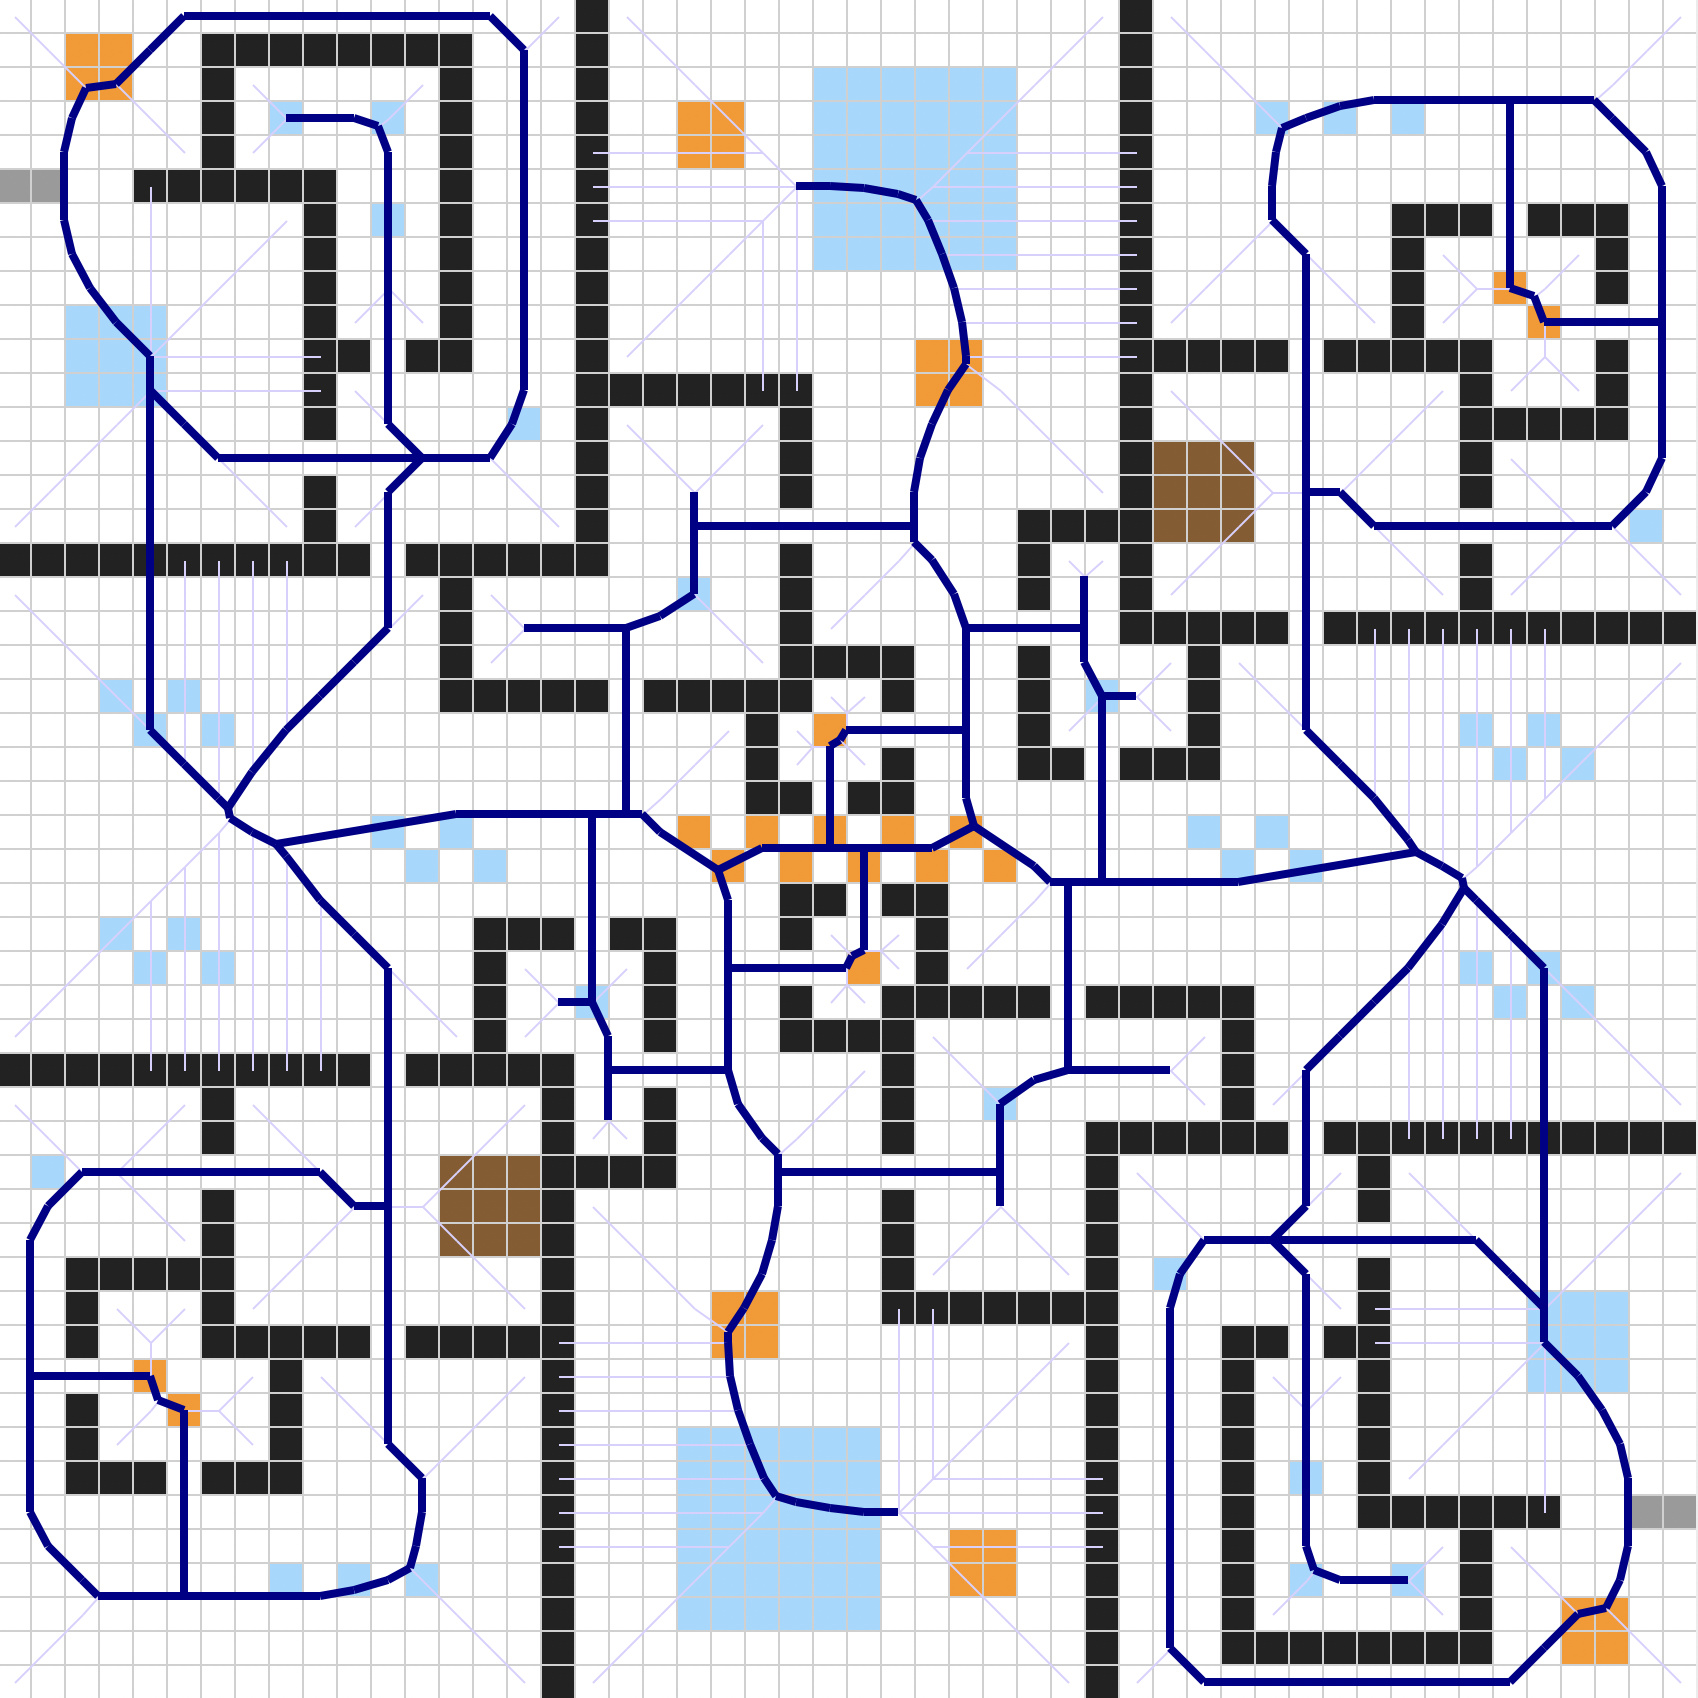
\includegraphics[width=\linewidth]{images/voronoi_pruned.png}\\
    {\small Pruned}
  \end{minipage}
  \caption{Graph Pruning}
  \Description{A side-by-side comparison of a before/after of the Voronoi pruning, revealing the medial line.}
\end{figure}

\subsection{Region Nodes}

After pruning, we identify region nodes. A region node is either a
topological junction or endpoint, or a locally maximal radius point. The
locally maximal points are important because a long corridor between two
rooms may have no graph junction at the room center. The maximum-clearance
point marks the room-like part of that chain.

\statefigure{images/regions.png}{Region Nodes}{}

\begin{lstlisting}
for v in graph.vertices:
    if degree(v) != 2:
        regions.add(v)
    elif radius[v] >= REGION_MIN_RADIUS:
        if no nearby vertex has radius >= radius[v]:
            regions.add(v)
\end{lstlisting}

The ``nearby'' test uses Chebyshev distance bounded by the candidate's own
radius. This makes the region test scale with local feature size: in a
large room, nearby maxima suppress each other, while in a narrow corridor,
small local bumps do not become separate regions.
\subsection{Choke Extraction}

Once region nodes are known, chokepoints are extracted by walking every
chain between two adjacent regions. Along each chain, the vertex with
minimum radius is the bottleneck.

\statefigure{images/chokepoint.png}{Chokepoints... ?}{}

Uh oh. That's a lot of chokepoints, including some we cannot feasibly block. We can get around this issue by merging nearby regions together to
remove some of the duplicate chokepoints we see.

The merge pass treats the region graph as a set of region nodes connected
by candidate chokepoints. A chokepoint is only useful if it is
substantially narrower than the regions it separates; otherwise it is more
like a harmless local wiggle in the medial graph than a place where placing
a blocker changes movement.

We process candidate chokepoints from widest to narrowest and maintain a
union-find over region nodes. If a choke is too wide relative to either of
the two adjacent regions, we merge those regions and delete the choke:

\begin{lstlisting}
parent = {region: region for region in region_nodes}

def find(v):
    while parent[v] != v:
        parent[v] = parent[parent[v]]
        v = parent[v]
    return v

def union(a, b):
    ra, rb = find(a), find(b)
    if ra == rb:
        return
    # keep the wider region as the representative
    if radius[ra] >= radius[rb]:
        parent[rb] = ra
    else:
        parent[ra] = rb
\end{lstlisting}

The main rule compares the choke radius against the radii of the two
regions it connects. If the bottleneck is close in size to the surrounding
regions, then it is not really a bottleneck, so the two regions should be
considered one larger region:

\begin{lstlisting}
for start, choke, end in chokes_by_decreasing_radius:
    r_start = find(start)
    r_end   = find(end)

    if r_start == r_end:
        remove(choke)
        continue

    choke_r = radius[choke]
    small_r = min(radius[r_start], radius[r_end])
    large_r = max(radius[r_start], radius[r_end])

    if (choke_r > ratio_small * small_r
            or choke_r > ratio_large * large_r):
        union(r_start, r_end)
        remove(choke)
\end{lstlisting}

This removes many duplicate chokepoints in open areas. For example, if two
large chambers are connected by several nearby shallow dips in radius, the
widest dips are merged away first, leaving only the narrowest meaningful
separator.

We also added a second rule for the common case where a small intermediate
region is created between two chokepoints. If a region has exactly two
active chokepoints and the larger of them is still too wide relative to the
region itself, we merge through it. This prevents tiny artificial regions
from producing pairs of redundant blockers:

\begin{lstlisting}
# after ignoring already-removed chokes
for region in (r_start, r_end):
    active = active_chokes_touching(region)

    if len(active) == 2:
        if max(radius[c] for c in active) > ratio_two_choke * radius[region]:
            union(r_start, r_end)
            remove(choke)
            break
\end{lstlisting}

\statefigure{images/chokepoint_merged.png}{After Merging}{}

After merging, any removed choke vertices are deleted from the choke set,
and rounded blocker placements are recomputed from the remaining chokes.


\begin{lstlisting}
for region in regions:
    for edge in outgoing_edges(region):
        path = walk_until_next_region(edge)

        if path reaches another region:
            choke = argmin(path, key=radius)
            if radius[choke] <= MAX_CHOKE_RADIUS:
                chokes.add((region, choke, other_region))
\end{lstlisting}

This gives us a graph-level interpretation of a chokepoint: it is the
narrowest point on a route between two larger spaces. That distinction is
what prevents every wall-adjacent pixel from being treated as important.

We then convert the geometric choke into an in-game blocker. Very narrow
chokes can be blocked by a single barrier. Wider chokes use a launcher,
because a launcher controls a larger effective area by throwing enemy
builders back out of the corridor.

\begin{lstlisting}
def blocker_kind(radius):
    if radius <= WALL_CHOKE_RADIUS:
        return BARRIER
    if radius <= LAUNCHER_CHOKE_RADIUS:
        return LAUNCHER
    return None
\end{lstlisting}

\statefigure{images/chokepoint_simplified.png}{Classify Launchers}{}

The geometric point is rounded back to a buildable tile. Candidates whose
rounded footprints overlap are clustered, and we keep the tightest choke
in each cluster.

\begin{lstlisting}
for choke in chokes:
    tile = round_to_tile(position[choke])
    kind = blocker_kind(radius[choke])
    if kind:
        candidates.append((tile, kind, radius[choke]))

clusters = overlap_clusters(candidates)
for cluster in clusters:
    keep min cluster by radius
\end{lstlisting}

\subsection{Using Chokepoints In-Game}

The chokepoint output is consumed passively by builders. We do not create
a dedicated ``chokepoint state'' with a high score ceiling, because
blocking terrain is useful opportunistically but should not override
obvious attacks, repairs, or routing work. Instead, after the main state
runs, the builder checks whether it can cheaply place a chokepoint blocker
nearby.
\vfill\null

\begin{lstlisting}
def try_passive_chokepoint_action_only():
    if action_on_cooldown:
        return False

    for choke in nearby_chokepoints():
        if already_blocked(choke):
            continue
        if can_build(choke.kind, choke.tile):
            build(choke.kind, choke.tile)
            return True

    return False
\end{lstlisting}

Launchers built at chokepoints use a specialized throw policy. Instead of
maximizing range, we attempt to get the opponent builder stuck walking back into the chokepoint infinitely. We hence launch to the last nth position they were seen.

\begin{lstlisting}
if launcher_is_chokepoint_launcher:
    enemy = best_enemy_builder_in_range()
    dest = position_from_enemy_history(enemy)
    if can_launch(enemy, dest):
        launch(enemy, dest)
\end{lstlisting}

This is especially effective when the enemy needs a builder to heal an
attack route or repair a broken conveyor. Throwing the builder backward
turns one launcher action into several turns of lost walking time.

\begin{figure}[htbp]
  \centering
  \begin{minipage}{0.48\linewidth}
    \centering
    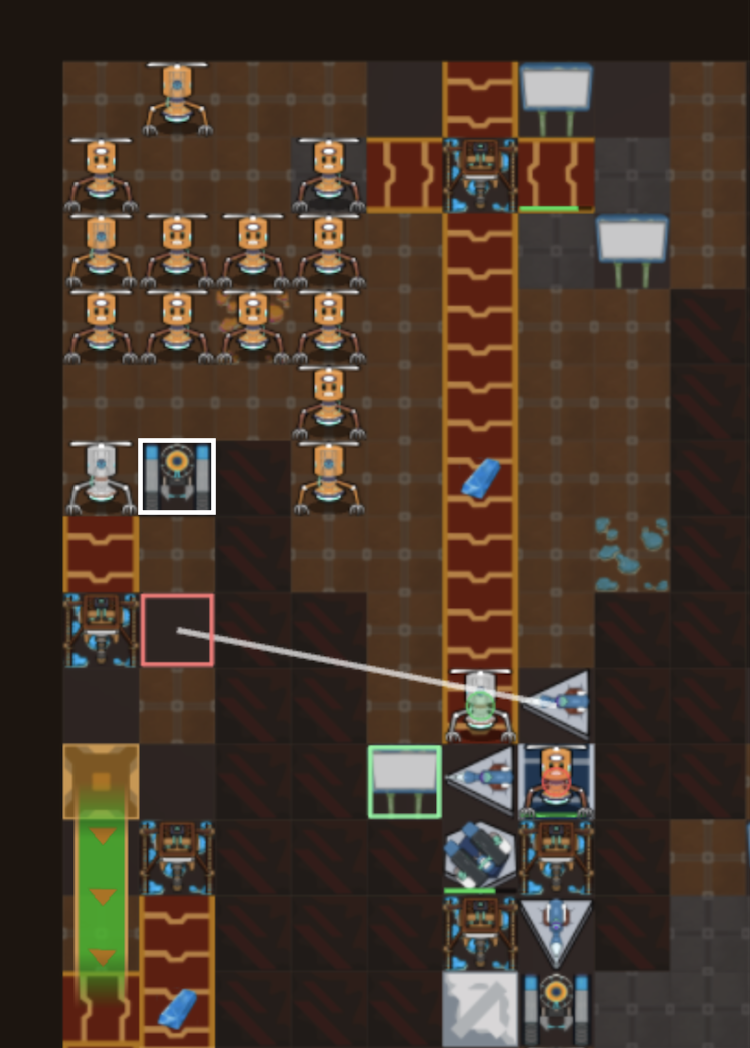
\includegraphics[width=\linewidth]{images/chokepoint_demo.png}\\
    {\small In Game}
  \end{minipage}
  \hfill
  \begin{minipage}{0.48\linewidth}
    \centering
    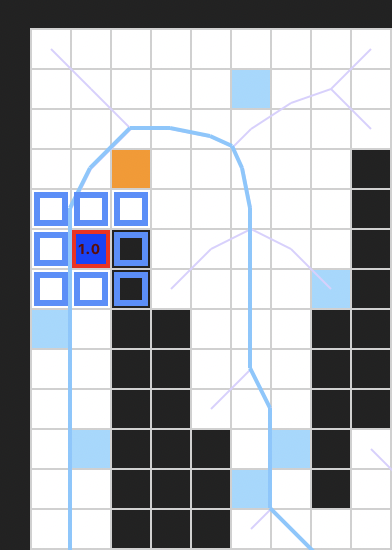
\includegraphics[width=\linewidth]{images/chokepoint_tooling_pad_crop2.png}\\
    {\small Tooling}
  \end{minipage}
  \caption{Chokepoint Blocks Opponent}
  \Description{A side-by-side comparison of tooling / in-game chokepoint calculation / execution}
\end{figure}

For instance, the figure above depicts a chokepoint launcher blocking a horde of opponent bots from healing or replacing a defensive building that was just broken; without the chokepoint launcher, they could easily have prevented this. However, our builder is able to move through freely and, a few turns later, place a turret.

\subsection{Incremental Execution}

The full detector is too expensive to recompute every turn. The in-game
version therefore runs as a resumable job. Each phase stores enough state
to continue later: obstacle components, boundary samples, Voronoi edges,
pruned graph state, and final blocker candidates.

\begin{lstlisting}
while budget_left() and job.phase != DONE:
    if job.phase == BUILD_GEOMETRY:
        job.build_some_components()
    elif job.phase == SAMPLE_BOUNDARY:
        job.sample_some_edges()
    elif job.phase == BUILD_GRAPH:
        job.process_some_voronoi_edges()
    elif job.phase == PRUNE:
        job.prune_some_leaves()
    elif job.phase == EXTRACT:
        job.extract_some_chokes()
\end{lstlisting}

This makes the computation compatible with the $2000\,\mu$s unit budget.
A builder can spend a small slice of time advancing the global chokepoint
job without risking timeout. Once the job finishes, all builders share the
same result.

\subsection{Medial-Axis Wall Reduction}

One optimization we added later was reducing certain wall polygons to
their medial axis before feeding them into the BWTA-style runtime. The
original boundary-sampling approach samples every exposed wall perimeter.
This is accurate, but large solid wall blobs can contribute many perimeter
segments whose fine detail has little strategic effect.

For sufficiently thick or compact wall components, we can replace the
component's full perimeter with a much smaller medial-axis
representative. Conceptually, instead of describing every pixel of the
wall outline, we describe the wall mass by its skeleton and local radius.
The surrounding free-space medial axis changes only slightly in these
cases, but the number of generated sites drops by a constant factor.

\begin{lstlisting}
for wall_component in components:
    if is_large_compact_component(wall_component):
        sites.extend(sample_wall_medial_axis(wall_component))
    else:
        sites.extend(sample_wall_perimeter(wall_component))
\end{lstlisting}

We only apply this reduction in cases where it is unlikely to remove a meaningful feature.
The optimization is therefore conservative: it is mainly a way to avoid oversampling large blocks of impassable terrain.

\section{Performance Optimization}

Runtime optimization of our bot was crucial not just to fit within the $2000\,\mu$s turn budget,
but also to free up time for our chokepoint calculations to run in the background.


\begin{table*}[t]
  \caption{The ten largest runtime consumers (ignoring chokepoint consumers), ranked by total self time.
    Self times are additive and sum to total CPU, so \% is each function's
    share of the total self time ($\approx\!6{,}483$\,ms over $6{,}070$
    profiled turns of one map); the listed ten account for $\approx\!35\%$.
    $\mu$s/call is mean self time per invocation.}
  \label{tab:profile}
  \footnotesize
  \begin{tabular}{lrrrr}
    \toprule
    Function                                   & Calls   & Self (ms) & $\mu$s/call & \%   \\
    \midrule
    \code{map\_info:update\_at}                & 470,546 & 883.9     & 1.9         & 13.6 \\
    \code{map\_info:update}                    & 6,070   & 336.7     & 55.5        & 5.2  \\
    \code{pathing:\_claim\_zone\_on\_passable} & 3,412   & 222.4     & 65.2        & 3.4  \\
    \code{map\_info:\_compute\_route\_targets} & 6,716   & 218.0     & 32.5        & 3.4  \\
    \code{pathing:bfs\_move}                   & 3,655   & 123.1     & 33.7        & 1.9  \\
    \code{map\_info:\_carrying\_expand}        & 5,321   & 117.8     & 22.1        & 1.8  \\
    \code{Controller.get\_tile\_building\_id}  & 414,358 & 113.2     & 0.27        & 1.7  \\
    \code{map\_info:expand\_chebyshev}         & 71,745  & 111.2     & 1.55        & 1.7  \\
    \code{pathing:\_closest\_impl}             & 15,170  & 84.3      & 5.56        & 1.3  \\
    \code{map\_info:update\_move}              & 2,752   & 76.6      & 27.8        & 1.2  \\
    \bottomrule
  \end{tabular}
\end{table*}

Table~\ref{tab:profile} shows that all of our top ten runtime callers deal with map info or pathfinding.

\subsection{Bitmasks}

One of our main optimizations was using bitmasks to store map info, since using bit operations on Python big integers was significantly faster than iterating over or indexing into arrays.

For example, we can iterate over all set bits in a mask using the canonical
two's-complement LSB idiom:

\begin{lstlisting}
while mask:
    lsb = mask & -mask        # isolate lowest set bit
    n = lsb.bit_length() - 1  # its position
    # ... use Position(n % W, n // W) ...
    mask ^= lsb               # clear and continue
\end{lstlisting}

Thus, if we build a mask containing possible target tiles (for explore targets, turret placements, etc.), the time complexity is proportional to the number of set bits rather than the number of tiles.

\subsection{Local Variable Hoisting}

Python attribute and global lookups are not free, and some of our inner loops
run hundreds of thousands of times per turn. Hence, every hot function binds the module and
controller members it needs to locals \emph{once}, before the loop:

\begin{lstlisting}
# bfs_move, before the frontier loop iterates:
bm_et = map_info._bm_et; 
nlc = map_info._not_left_col;
board = map_info._board_mask; 
bcost = barrier_cost;
# update_at, binding hot Controller methods to locals:
get_tile_env         = rc.get_tile_env
get_tile_building_id = rc.get_tile_building_id
get_hp               = rc.get_hp
\end{lstlisting}

\subsection{Integer-Indexed Tables}

\code{cambc} enums are not integer-valued, so using them as dictionary
keys or in \code{frozenset} membership tests costs a hash per access.
\code{map\_info} converts every enum to a sequential index once at import
and thereafter uses list indexing and boolean lookup tables instead of dictionary lookups.

\subsection{Caching and Memoization}

Many of our derived bitmasks, calculated targets, etc., are memoized on the map info structures they depend on.
Hence, we limit recomputation to when relevant infrastructure changes.

We also memoize some calculations irrespective of local map changes.
The harvest zone, which is a Voronoi floodfill from our core against the predicted
enemy core used to approximate safe harvest locations, only runs when symmetry predictions update.
The column and row guard masks and the eight per-facing direction
templates for sentinels are likewise built at
\code{init} and not touched again.

\subsection{Incremental Updates}

We also prioritize patching information rather than fully rebuilding it.
\code{update\_at} maintains conveyor output and reverse conveyor output bitmasks as buildings are updated,
rather than rescanning the entire map.

Furthermore, after a move, \code{update\_move} diffs the old and
new vision masks and calls \code{update\_at} only on tiles that became
visible:

\begin{lstlisting}
for tile in nearby:
    bit = 1 << (tile.x + tile.y * W)
    new_visible |= bit
    if not (old_visible & bit):   # only the delta
        update_at(tile)
\end{lstlisting}

This reduces the number of tiles we scan after moving from all tiles within vision to only the newly discovered tiles.

\subsection{TTL Caches}

States that depend on expensive build paths remember failure. Bounded-TTL
sets include caches for harvest failures, unaffordable attempts, secure
failures, attack failures, and pathing failures,
which record ``this tile was unbuildable or unaffordable'' for $\sim\!100$
rounds, so a bot does not waste runtime trying to recompute if a previously failed
target tile should be acted on again.

\subsection{Debugging}

\code{log.py} binds \code{log} at module load to one of two definitions
depending on a single boolean:

\begin{lstlisting}
DEBUG_LOGGING = False
if DEBUG_LOGGING:
    def log(*args, **kwargs): print(*args, **kwargs)
else:
    def log(*args, **kwargs): pass
\end{lstlisting}

Every \code{log(...)} call site thus becomes a no-op function call when we turn the flag off before submitting our bot.

\section{Conclusion}

Overall, our final bot uses a memoryless approach, backed
by a robust map info layer and caching system, to decide on the best set of actions for
any given turn. This allows our builder bots to adapt quickly to changing circumstances and allows for complex behavior to emerge.

\end{document}
